% !TEX program = xelatex
\documentclass[11pt,a4paper]{article}

\usepackage{fontspec}
\usepackage{polyglossia}
\setmainlanguage{greek}
\setotherlanguage{english}
\setmainfont{DejaVu Serif}[Scale=0.95]
\setsansfont{DejaVu Sans}[Scale=0.95]
\setmonofont{DejaVu Sans Mono}[Scale=0.85]

\usepackage[a4paper, margin=2.35cm]{geometry}
\usepackage{amsmath, amssymb}
\usepackage{booktabs}
\usepackage{array}
\usepackage{longtable}
\usepackage{xcolor}
\usepackage{listings}
\usepackage[hidelinks]{hyperref}
\usepackage{enumitem}
\usepackage{caption}
\usepackage{graphicx}
\usepackage{float}

\definecolor{codebg}{HTML}{F5F5F5}
\definecolor{darkblue}{HTML}{164E63}

\lstset{
    basicstyle=\ttfamily\footnotesize,
    breaklines=true,
    frame=single,
    backgroundcolor=\color{codebg},
    columns=fullflexible,
    keepspaces=true,
    language=Python
}

\setlist[itemize]{leftmargin=1.35cm}
\setlist[enumerate]{leftmargin=1.35cm}
\newcommand{\code}[1]{\texttt{#1}}
\newcommand{\eng}[1]{\textenglish{#1}}

\title{\textbf{Επεξηγηματικό Report 3ης Εργασίας}\\[4pt]
\large Ερώτημα Α (a)-(c) και Ερώτημα Β: Logistic Regression, LDA, QDA, Gaussian NB και KNN}
\author{ΑΕΜ: 6931}
\date{Απρίλιος 2026}

\begin{document}
\maketitle
\tableofcontents
\newpage

\section{Ποιο κομμάτι της εργασίας λύνουμε εδώ}

Η 3η εργασία μάς δίνει ένα σύνολο δεδομένων με κρασιά. Κάθε γραμμή του
αρχείου αντιστοιχεί σε ένα κρασί και κάθε στήλη περιγράφει κάποιο χημικό
χαρακτηριστικό του, όπως το \code{alcohol}, το \code{pH}, τα \code{chlorides}
κ.λπ. Υπάρχει επίσης η στήλη \code{wine\_type}, η οποία λέει αν το κρασί είναι
\code{white} ή \code{red}.

\subsection{Η εκφώνηση, με απλά λόγια}

Η εκφώνηση ζητά να προβλέψουμε τον τύπο του κρασιού:
\[
\text{wine\_type} \in \{\text{red}, \text{white}\}.
\]
Δηλαδή, θέλουμε να φτιάξουμε ένα μοντέλο που να κοιτάζει κάποια χημική
μέτρηση ενός κρασιού και να απαντά:
\[
\text{``Πιστεύω ότι αυτό το κρασί είναι κόκκινο ή λευκό.''}
\]

Πριν εκπαιδεύσουμε οποιοδήποτε μοντέλο, πρέπει να χωρίσουμε τα δεδομένα σε:
\begin{itemize}
    \item \textbf{training set} 70\%: τα δεδομένα από τα οποία το μοντέλο
    μαθαίνει.
    \item \textbf{test set} 30\%: τα δεδομένα που κρατάμε στην άκρη για
    να ελέγξουμε αν το μοντέλο έμαθε κάτι χρήσιμο.
\end{itemize}

Ο χωρισμός γίνεται με \code{random\_state = 6931}, δηλαδή με seed ίσο με τον
ΑΕΜ. Αυτό σημαίνει ότι όποτε ξανατρέξουμε τον κώδικα, θα πάρουμε ακριβώς τον
ίδιο διαχωρισμό σε training και test. Άρα τα αποτελέσματα είναι
αναπαραγώγιμα.

\subsection{Τι είναι το Ερώτημα Α}

Το Ερώτημα Α ζητά να κάνουμε πρόβλεψη του τύπου κρασιού χρησιμοποιώντας
\textbf{μία μόνο προβλεπτική μεταβλητή κάθε φορά}. Οι τρεις μεταβλητές που
εξετάζονται είναι:
\begin{enumerate}
    \item \code{alcohol}
    \item \code{pH}
    \item \code{chlorides}
\end{enumerate}

Για κάθε μία από αυτές, η εργασία ζητά να εφαρμόσουμε τρεις μεθόδους
ταξινόμησης:
\begin{enumerate}
    \item Logistic Regression
    \item Linear Discriminant Analysis
    \item Gaussian Naive Bayes
\end{enumerate}

Σε αυτό το report καλύπτουμε τα τρία πρώτα υποερωτήματα του Ερωτήματος Α:
\textbf{Α(a) Logistic Regression}, \textbf{Α(b) Linear Discriminant
Analysis} και \textbf{Α(c) Gaussian Naive Bayes}. Άρα κάνουμε πρώτα τρία
πειράματα με Logistic Regression:
\[
\begin{array}{ll}
1. & \text{Logistic Regression με μοναδική μεταβλητή το alcohol} \\
2. & \text{Logistic Regression με μοναδική μεταβλητή το pH} \\
3. & \text{Logistic Regression με μοναδική μεταβλητή τα chlorides}
\end{array}
\]
και έπειτα τα ίδια τρία πειράματα με LDA:
\[
\begin{array}{ll}
1. & \text{LDA με μοναδική μεταβλητή το alcohol} \\
2. & \text{LDA με μοναδική μεταβλητή το pH} \\
3. & \text{LDA με μοναδική μεταβλητή τα chlorides}
\end{array}
\]
και τέλος τα ίδια τρία πειράματα με Gaussian Naive Bayes:
\[
\begin{array}{ll}
1. & \text{Gaussian NB με μοναδική μεταβλητή το alcohol} \\
2. & \text{Gaussian NB με μοναδική μεταβλητή το pH} \\
3. & \text{Gaussian NB με μοναδική μεταβλητή τα chlorides}
\end{array}
\]

Για κάθε πείραμα υπολογίζουμε:
\begin{itemize}
    \item τον \textbf{confusion matrix} στα test δεδομένα,
    \item την \textbf{accuracy},
    \item την \textbf{balanced accuracy},
    \item το \textbf{recall} για λευκά και κόκκινα κρασιά,
    \item το \textbf{precision},
    \item το \textbf{F1-score},
    \item και την \textbf{AUC}.
\end{itemize}

\section{Θεωρητικό υπόβαθρο}

\subsection{Τι σημαίνει ``πρόβλεψη τύπου κρασιού''}

Στα δεδομένα μας η στήλη που θέλουμε να προβλέψουμε είναι η \code{wine\_type}.
Αυτή ονομάζεται \textbf{μεταβλητή στόχος} ή \textbf{target variable}. Οι
στήλες που χρησιμοποιούμε για να τη μαντέψουμε ονομάζονται
\textbf{προβλεπτικές μεταβλητές} ή \textbf{features}.

Εδώ η μεταβλητή στόχος έχει δύο δυνατές κατηγορίες:
\[
\text{red}, \quad \text{white}.
\]
Όταν θέλουμε να προβλέψουμε κατηγορία, δεν κάνουμε απλή αριθμητική πρόβλεψη.
Κάνουμε \textbf{ταξινόμηση} (\eng{classification}).

Παράδειγμα:
\begin{itemize}
    \item Αν θέλαμε να προβλέψουμε την τιμή \code{alcohol = 11.2}, θα είχαμε
    πρόβλημα παλινδρόμησης.
    \item Αν θέλουμε να προβλέψουμε αν το κρασί είναι \code{red} ή
    \code{white}, έχουμε πρόβλημα ταξινόμησης.
\end{itemize}

Η Logistic Regression, παρότι έχει τη λέξη ``Regression'' στο όνομα, εδώ
χρησιμοποιείται ως \textbf{μέθοδος ταξινόμησης}. Αυτό στην αρχή φαίνεται
παράξενο, αλλά ο λόγος είναι ότι δεν προβλέπει κατευθείαν την κατηγορία.
Πρώτα προβλέπει μια \textbf{πιθανότητα}.

\subsection{Πώς κωδικοποιούμε τις δύο κατηγορίες}

Οι αλγόριθμοι μηχανικής μάθησης δουλεύουν πιο εύκολα με αριθμούς παρά με
λέξεις. Γι' αυτό μετατρέπουμε το \code{wine\_type} ως εξής:
\[
\text{red} = 0, \qquad \text{white} = 1.
\]

Με αυτή τη σύμβαση, όταν το μοντέλο δίνει πιθανότητα, η πιθανότητα αυτή
διαβάζεται ως:
\[
P(\text{white} \mid x).
\]
Δηλαδή:
\begin{quote}
``Ποια είναι η πιθανότητα το κρασί να είναι λευκό, αν ξέρω την τιμή της
μεταβλητής \(x\);''
\end{quote}

Το \(x\) εδώ είναι κάθε φορά μία από τις μεταβλητές:
\[
x = \text{alcohol}, \quad x = \text{pH}, \quad x = \text{chlorides}.
\]

\subsection{Τι κάνει η Logistic Regression}

Η Logistic Regression προσπαθεί να συνδέσει μία μεταβλητή \(x\) με την
πιθανότητα ένα κρασί να είναι λευκό. Η σχέση δεν γράφεται απευθείας ως
ευθεία πάνω στην πιθανότητα, γιατί οι πιθανότητες πρέπει πάντα να μένουν
μεταξύ 0 και 1.

Αν γράφαμε κάτι σαν:
\[
P(\text{white}) = \beta_0 + \beta_1 x,
\]
τότε η δεξιά πλευρά θα μπορούσε να βγει μικρότερη από 0 ή μεγαλύτερη από 1.
Αυτό δεν γίνεται να είναι πιθανότητα.

Η Logistic Regression λύνει αυτό το πρόβλημα με τη συνάρτηση sigmoid:
\[
P(\text{white} \mid x) =
\frac{1}{1 + e^{-(\beta_0 + \beta_1 x)}}.
\]

Η ποσότητα:
\[
z = \beta_0 + \beta_1 x
\]
μπορεί να πάρει οποιαδήποτε τιμή, από \(-\infty\) μέχρι \(+\infty\). Η sigmoid
παίρνει αυτόν τον αριθμό και τον μετατρέπει σε πιθανότητα μεταξύ 0 και 1.

\subsection{Πώς αποφασίζει τελικά red ή white}

Αφού υπολογιστεί η πιθανότητα \(P(\text{white} \mid x)\), χρειαζόμαστε έναν
κανόνα απόφασης. Ο συνηθισμένος κανόνας είναι:
\[
\begin{cases}
\text{πρόβλεψη white}, & \text{αν } P(\text{white} \mid x) \ge 0.5,\\
\text{πρόβλεψη red}, & \text{αν } P(\text{white} \mid x) < 0.5.
\end{cases}
\]

Το \(0.5\) λέγεται \textbf{κατώφλι απόφασης} (\eng{decision threshold}).
Σημαίνει απλά:
\begin{quote}
Αν το μοντέλο πιστεύει ότι η πιθανότητα για white είναι τουλάχιστον 50\%,
τότε προβλέπει white. Αλλιώς προβλέπει red.
\end{quote}

Αυτό το σημείο είναι πολύ σημαντικό για την ερμηνεία των αποτελεσμάτων μας.
Ένα μοντέλο μπορεί να κατατάσσει σχετικά καλά τα κρασιά από ``πιο πιθανό
λευκό'' προς ``πιο πιθανό κόκκινο'', αλλά αν οι πιθανότητες σπάνια πέφτουν
κάτω από 0.5, τότε με το default κατώφλι θα προβλέπει σχεδόν πάντα white.

\subsection{Γιατί χωρίζουμε σε training και test}

Αν εκπαιδεύαμε και αξιολογούσαμε το μοντέλο στα ίδια δεδομένα, θα ήταν σαν να
βάζαμε σε έναν μαθητή ακριβώς τα ίδια θέματα που είχε δει στην προετοιμασία.
Δεν θα ξέραμε αν πραγματικά κατάλαβε ή αν απλώς ``θυμήθηκε'' τα παραδείγματα.

Γι' αυτό κάνουμε:
\[
70\% \text{ training}, \qquad 30\% \text{ test}.
\]

Το μοντέλο βλέπει μόνο το training set. Το test set το βλέπει μόνο στο τέλος,
όταν θέλουμε να μετρήσουμε την απόδοση.

Στη δική μας ανάλυση:
\begin{itemize}
    \item συνολικά δεδομένα: 5.295 κρασιά,
    \item training set: 3.706 κρασιά,
    \item test set: 1.589 κρασιά.
\end{itemize}

Η κατανομή των κλάσεων στο συνολικό dataset είναι:
\[
\text{white}: 3991 \; (75{,}37\%), \qquad
\text{red}: 1304 \; (24{,}63\%).
\]

Άρα το dataset είναι \textbf{ανισόρροπο}: υπάρχουν περίπου τριπλάσια λευκά
κρασιά από κόκκινα. Αυτό έχει τεράστια σημασία, γιατί ένα πολύ απλοϊκό
μοντέλο που προβλέπει πάντα \code{white} θα έχει ήδη accuracy περίπου 75\%.
Επομένως, η accuracy μόνη της μπορεί να μας ξεγελάσει.

\subsection{Τι είναι ο confusion matrix}

Ο \textbf{confusion matrix} είναι ένας πίνακας που δείχνει πόσες προβλέψεις
ήταν σωστές και πόσες λάθος. Επειδή έχουμε δύο κλάσεις, ο πίνακας έχει 2
γραμμές και 2 στήλες.

Στο report χρησιμοποιούμε τη διάταξη:
\[
\begin{array}{c|cc}
 & \text{pred red} & \text{pred white} \\
\hline
\text{true red} & TN & FP \\
\text{true white} & FN & TP
\end{array}
\]

Οι γραμμές δείχνουν την πραγματική κατηγορία. Οι στήλες δείχνουν την
πρόβλεψη του μοντέλου.

Με τη σύμβαση \code{white = 1}, η θετική κλάση είναι το white. Άρα:
\begin{itemize}
    \item \textbf{TN} (\eng{True Negative}): πραγματικά red και προβλέφθηκαν
    red.
    \item \textbf{FP} (\eng{False Positive}): πραγματικά red αλλά
    προβλέφθηκαν white.
    \item \textbf{FN} (\eng{False Negative}): πραγματικά white αλλά
    προβλέφθηκαν red.
    \item \textbf{TP} (\eng{True Positive}): πραγματικά white και
    προβλέφθηκαν white.
\end{itemize}

\subsection{Τα μέτρα αξιολόγησης}

\subsubsection{Accuracy}

Η accuracy είναι το ποσοστό όλων των σωστών προβλέψεων:
\[
\text{Accuracy} =
\frac{TP + TN}{TP + TN + FP + FN}.
\]

Είναι εύκολο μέτρο, αλλά σε ανισόρροπα δεδομένα μπορεί να είναι
παραπλανητικό. Στο δικό μας dataset, επειδή τα white είναι 75\%, ένα μοντέλο
που λέει πάντα white θα έχει περίπου 75\% accuracy χωρίς να ξεχωρίζει
καθόλου τα κόκκινα κρασιά.

\subsubsection{Sensitivity για white}

Το sensitivity για white, δηλαδή το recall της θετικής κλάσης, δείχνει:
\begin{quote}
Από όλα τα πραγματικά λευκά κρασιά, πόσα βρήκε σωστά το μοντέλο;
\end{quote}

\[
\text{Sensitivity}_{white} =
\frac{TP}{TP + FN}.
\]

\subsubsection{Specificity για red}

Το specificity για red δείχνει:
\begin{quote}
Από όλα τα πραγματικά κόκκινα κρασιά, πόσα βρήκε σωστά το μοντέλο;
\end{quote}

\[
\text{Specificity}_{red} =
\frac{TN}{TN + FP}.
\]

Αυτό το μέτρο είναι κρίσιμο εδώ, γιατί τα κόκκινα κρασιά είναι η μειοψηφική
κλάση. Αν το specificity είναι 0, τότε το μοντέλο δεν αναγνωρίζει κανένα
κόκκινο κρασί.

\subsubsection{Balanced accuracy}

Η balanced accuracy είναι ο μέσος όρος του recall για τις δύο κλάσεις:
\[
\text{Balanced Accuracy} =
\frac{\text{Sensitivity}_{white} + \text{Specificity}_{red}}{2}.
\]

Αν ένα μοντέλο προβλέπει πάντα white:
\[
\text{Sensitivity}_{white} = 1, \qquad
\text{Specificity}_{red} = 0,
\]
άρα:
\[
\text{Balanced Accuracy} = \frac{1 + 0}{2} = 0.5.
\]

Το 0.5 εδώ σημαίνει πρακτικά ότι το μοντέλο δεν κάνει ουσιαστική
ταξινόμηση και λειτουργεί σαν ένας ταξινομητής που ευνοεί μόνο την
πλειοψηφική κλάση.

\subsubsection{Precision και F1-score}

Το precision απαντά στην ερώτηση:
\begin{quote}
Όταν το μοντέλο προβλέπει μια κλάση, πόσο συχνά έχει δίκιο;
\end{quote}

Για παράδειγμα, το precision για red δείχνει πόσα από τα κρασιά που
προβλέφθηκαν ως red ήταν πράγματι red.

Το F1-score συνδυάζει precision και recall:
\[
F1 = 2 \cdot
\frac{\text{Precision} \cdot \text{Recall}}
{\text{Precision} + \text{Recall}}.
\]

Αν ένα μοντέλο δεν προβλέπει ποτέ red, τότε το F1 για red γίνεται 0.

\subsubsection{ROC καμπύλη και AUC}

Πριν εξηγήσουμε την AUC, πρέπει πρώτα να εξηγήσουμε τι είναι η
\textbf{ROC καμπύλη}. Η ROC καμπύλη δεν είναι άλλη μία τελική πρόβλεψη του
μοντέλου. Είναι ένας τρόπος να δούμε πώς συμπεριφέρεται το μοντέλο όταν
αλλάζουμε το κατώφλι απόφασης.

Μέχρι τώρα χρησιμοποιούσαμε το συνηθισμένο κατώφλι 0.5:
\[
\begin{cases}
\text{white}, & \text{αν } P(\text{white}) \ge 0.5,\\
\text{red}, & \text{αν } P(\text{white}) < 0.5.
\end{cases}
\]

Όμως το 0.5 δεν είναι ο μόνος δυνατός κανόνας. Θα μπορούσαμε να είμαστε πιο
αυστηροί και να πούμε:
\[
\text{Πρόβλεψε white μόνο αν } P(\text{white}) \ge 0.8.
\]
Ή θα μπορούσαμε να είμαστε πιο χαλαροί και να πούμε:
\[
\text{Πρόβλεψε white αν } P(\text{white}) \ge 0.3.
\]

Κάθε διαφορετικό κατώφλι αλλάζει τις τελικές προβλέψεις. Αν χαμηλώσουμε το
κατώφλι, το μοντέλο προβλέπει πιο εύκολα white. Αν ανεβάσουμε το κατώφλι,
το μοντέλο γίνεται πιο αυστηρό και προβλέπει λιγότερα white.

Η ROC καμπύλη δοκιμάζει πολλά τέτοια κατώφλια και για κάθε κατώφλι υπολογίζει
δύο ποσότητες:
\[
\text{True Positive Rate} =
\frac{TP}{TP + FN}
\]
και
\[
\text{False Positive Rate} =
\frac{FP}{FP + TN}.
\]

Στο δικό μας πρόβλημα, επειδή έχουμε ορίσει \code{white = 1}, το
\textbf{True Positive Rate} είναι το recall των white κρασιών:
\begin{quote}
Από όλα τα πραγματικά white, πόσα αναγνωρίστηκαν ως white;
\end{quote}

Το \textbf{False Positive Rate} δείχνει πόσα red κρασιά μπερδεύτηκαν ως
white:
\begin{quote}
Από όλα τα πραγματικά red, πόσα προβλέφθηκαν λανθασμένα ως white;
\end{quote}

Άρα η ROC καμπύλη είναι ένα γράφημα με:
\[
x\text{-άξονας} = \text{False Positive Rate},
\qquad
y\text{-άξονας} = \text{True Positive Rate}.
\]

Ιδανικά θέλουμε το μοντέλο να έχει υψηλό True Positive Rate και χαμηλό False
Positive Rate. Δηλαδή θέλουμε να βρίσκει πολλά white χωρίς να μπερδεύει πολλά
red ως white.

\paragraph{Πώς δημιουργείται βήμα-βήμα η ROC καμπύλη.}
Το μοντέλο Logistic Regression δεν δίνει μόνο την τελική κατηγορία
\code{red} ή \code{white}. Για κάθε κρασί δίνει πρώτα μια πιθανότητα, π.χ.
\[
P(\text{white}) = 0{,}91, \quad
P(\text{white}) = 0{,}74, \quad
P(\text{white}) = 0{,}42.
\]

Η ROC καμπύλη φτιάχνεται σαν να βάζουμε όλα τα κρασιά σε μια σειρά, από αυτό
που το μοντέλο θεωρεί πιο πιθανό να είναι white μέχρι αυτό που θεωρεί λιγότερο
πιθανό να είναι white. Μετά μετακινούμε σταδιακά το κατώφλι από πολύ αυστηρό
σε πολύ χαλαρό.

\begin{itemize}
    \item Αν το κατώφλι είναι πάρα πολύ ψηλά, π.χ. πάνω από όλες τις
    πιθανότητες, τότε το μοντέλο δεν προβλέπει κανένα κρασί ως white.
    Άρα δεν βρίσκει κανένα white, αλλά δεν κάνει και κανένα red λάθος ως
    white. Το σημείο της ROC είναι:
    \[
    (FPR, TPR) = (0, 0).
    \]

    \item Όσο χαμηλώνουμε το κατώφλι, αρχίζουν να προβλέπονται κάποια κρασιά
    ως white. Αν αυτά που προστίθενται είναι πράγματι white, τότε αυξάνεται
    το \(TPR\), δηλαδή η καμπύλη ανεβαίνει προς τα πάνω.

    \item Αν όμως αυτά που προστίθενται είναι red που το μοντέλο τα μπερδεύει
    ως white, τότε αυξάνεται το \(FPR\), δηλαδή η καμπύλη κινείται προς τα
    δεξιά.

    \item Αν το κατώφλι γίνει πάρα πολύ χαμηλό, τότε το μοντέλο προβλέπει όλα
    τα κρασιά ως white. Τότε έχει βρει όλα τα πραγματικά white, αλλά έχει
    μπερδέψει και όλα τα red ως white. Το τελευταίο σημείο είναι:
    \[
    (FPR, TPR) = (1, 1).
    \]
\end{itemize}

Άρα η ROC καμπύλη ξεκινά πάντα από το κάτω αριστερό σημείο \((0,0)\) και
καταλήγει πάντα στο πάνω δεξί σημείο \((1,1)\). Η σημαντική πληροφορία δεν
είναι απλώς από πού ξεκινά και πού τελειώνει, αλλά \textbf{ποια διαδρομή}
ακολουθεί ενδιάμεσα.

\paragraph{Γιατί παίρνει τη μορφή που παίρνει.}
Η μορφή της ROC καμπύλης δείχνει τη σειρά με την οποία το μοντέλο ``μαζεύει''
τα white και τα red καθώς χαμηλώνει το κατώφλι.

\begin{itemize}
    \item Αν το μοντέλο είναι \textbf{καλό}, τότε δίνει υψηλές πιθανότητες
    white κυρίως στα πραγματικά white κρασιά. Άρα, στην αρχή που χαμηλώνουμε
    το κατώφλι, προστίθενται πολλά σωστά white και λίγα λάθος red. Η καμπύλη
    ανεβαίνει γρήγορα προς τα πάνω και μένει κοντά στην πάνω αριστερή γωνία.

    \item Αν το μοντέλο είναι \textbf{τυχαίο}, τότε τα white και τα red είναι
    ανακατεμένα στη σειρά πιθανοτήτων. Καθώς χαμηλώνουμε το κατώφλι,
    προστίθενται περίπου με τον ίδιο ρυθμό σωστά white και λάθος red. Τότε η
    ROC μοιάζει με διαγώνια γραμμή από το \((0,0)\) στο \((1,1)\).

    \item Αν το μοντέλο είναι \textbf{τέλειο}, τότε όλα τα πραγματικά white
    έχουν μεγαλύτερη πιθανότητα από όλα τα πραγματικά red. Η καμπύλη ανεβαίνει
    πρώτα κάθετα μέχρι το \((0,1)\) και μετά πηγαίνει οριζόντια μέχρι το
    \((1,1)\).
\end{itemize}

Στην πράξη, επειδή έχουμε πεπερασμένο αριθμό κρασιών στο test set, η ROC δεν
είναι μια τέλεια λεία καμπύλη. Είναι περισσότερο μια κλιμακωτή γραμμή:
κάθε φορά που το κατώφλι περνάει την πιθανότητα ενός συγκεκριμένου κρασιού,
αλλάζει λίγο ο confusion matrix και άρα αλλάζει λίγο το \(TPR\) ή το \(FPR\).

\paragraph{Σύνδεση με τις δικές μας μεταβλητές.}
Στη Logistic Regression με μία μεταβλητή, η μορφή της ROC εξαρτάται από το
πόσο καλά χωρίζονται οι τιμές αυτής της μεταβλητής ανάμεσα στα red και white
κρασιά.

Για το \code{alcohol}, οι τιμές των red και white επικαλύπτονται πολύ. Το
μοντέλο δυσκολεύεται να βάλει πρώτα τα white και μετά τα red, οπότε η ROC
είναι κοντά στη διαγώνιο και η AUC βγαίνει κοντά στο 0,5.

Για το \code{pH}, υπάρχει κάποια διαφορά ανάμεσα στις δύο κλάσεις, αλλά όχι
πολύ καθαρή. Γι' αυτό η ROC είναι καλύτερη από τη διαγώνιο, αλλά όχι κοντά
στην ιδανική πάνω αριστερή γωνία.

Για τα \code{chlorides}, οι τιμές ξεχωρίζουν πολύ καλύτερα τα δύο είδη
κρασιού. Πολλά white παίρνουν υψηλότερη πιθανότητα white από πολλά red. Έτσι
η ROC ανεβαίνει γρήγορα προς τα πάνω και η AUC γίνεται πολύ υψηλή.

Η \textbf{AUC} σημαίνει \eng{Area Under the Curve}, δηλαδή
\textbf{εμβαδό κάτω από την ROC καμπύλη}. Άρα, πιο σωστά:
\begin{itemize}
    \item η \textbf{ROC} είναι η καμπύλη,
    \item η \textbf{AUC} είναι ένας αριθμός που συνοψίζει αυτή την καμπύλη.
\end{itemize}

Για να την καταλάβουμε διαισθητικά:
\begin{quote}
Η AUC μετρά πόσο καλά το μοντέλο μπορεί να βάλει τα white και red κρασιά
σε σωστή σειρά, από πιο πιθανό white προς λιγότερο πιθανό white.
\end{quote}

Μια AUC κοντά στο 0.5 σημαίνει ότι το μοντέλο δεν ξεχωρίζει τις δύο κλάσεις.
Μια AUC κοντά στο 1 σημαίνει πολύ καλή διακριτική ικανότητα.

Η AUC είναι χρήσιμη γιατί δεν εξαρτάται από το συγκεκριμένο κατώφλι 0.5.
Μπορεί λοιπόν να είναι υψηλή ακόμη κι αν το default κατώφλι δεν δίνει
ιδανικές τελικές προβλέψεις.

\section{Πώς λύσαμε το υποερώτημα Α(a)}

\subsection{Βήμα 1: Φόρτωση των δεδομένων}

Φορτώσαμε το αρχείο:
\[
\code{Data Analysis\_2026 3rd Case\_Data.csv}
\]
το οποίο βρίσκεται στον φάκελο της 3ης εργασίας. Η εκφώνηση λέει ότι αυτά
τα δεδομένα δεν χρειάζονται καθαρισμό, άρα δεν κάναμε διαδικασία διόρθωσης
λαθών όπως στην 1η εργασία.

\begin{lstlisting}
import pandas as pd

df = pd.read_csv("Data Analysis_2026 3rd Case_Data.csv")
\end{lstlisting}

\subsection{Βήμα 2: Ορισμός στόχου}

Η μεταβλητή στόχος είναι η \code{wine\_type}. Τη μετατρέψαμε σε αριθμητική:

\begin{lstlisting}
y = (df["wine_type"] == "white").astype(int)
\end{lstlisting}

Αυτό σημαίνει:
\[
\text{white} = 1, \qquad \text{red} = 0.
\]

\subsection{Βήμα 3: Επιλογή μίας προβλεπτικής μεταβλητής κάθε φορά}

Για το υποερώτημα Α(a), εκπαιδεύσαμε τρία ξεχωριστά μοντέλα Logistic
Regression:

\begin{lstlisting}
predictors = ["alcohol", "pH", "chlorides"]
\end{lstlisting}

Κάθε μοντέλο βλέπει μόνο μία στήλη. Για παράδειγμα, όταν εξετάζουμε το
\code{alcohol}, το μοντέλο δεν βλέπει ούτε \code{pH}, ούτε \code{chlorides},
ούτε καμία άλλη χημική μεταβλητή.

Αυτό γίνεται επειδή το Ερώτημα Α θέλει να δούμε πόσο χρήσιμη είναι κάθε
μεταβλητή \textbf{μόνη της}.

\subsection{Βήμα 4: Διαχωρισμός σε training και test}

Χρησιμοποιήσαμε:
\[
70\% \text{ training}, \qquad 30\% \text{ test},
\]
με:
\[
\code{random\_state = 6931}.
\]

Επιπλέον χρησιμοποιήθηκε \code{stratify=y}. Αυτό σημαίνει ότι ο χωρισμός
κρατά περίπου την ίδια αναλογία red/white και στο training και στο test.
Χωρίς stratification, θα μπορούσε τυχαία το test set να έχει λίγο
διαφορετική σύνθεση κλάσεων, κάτι που θα έκανε την αξιολόγηση λιγότερο
σταθερή.

\begin{lstlisting}
from sklearn.model_selection import train_test_split

X_train, X_test, y_train, y_test = train_test_split(
    X,
    y,
    test_size=0.30,
    random_state=6931,
    stratify=y
)
\end{lstlisting}

Με αυτόν τον χωρισμό προέκυψε:

\begin{center}
\begin{tabular}{lccc}
\toprule
Σύνολο & Πλήθος & red & white \\
\midrule
Training set & 3706 & 913 & 2793 \\
Test set & 1589 & 391 & 1198 \\
\bottomrule
\end{tabular}
\end{center}

\subsection{Βήμα 5: Εκπαίδευση Logistic Regression}

Για κάθε προβλεπτική μεταβλητή εκπαιδεύσαμε ένα μοντέλο:

\begin{lstlisting}
from sklearn.linear_model import LogisticRegression

model = LogisticRegression(solver="lbfgs", max_iter=1000)
model.fit(X_train, y_train)
\end{lstlisting}

Το \code{fit} είναι το σημείο όπου το μοντέλο μαθαίνει τις παραμέτρους
\(\beta_0\) και \(\beta_1\).

\subsection{Βήμα 6: Πρόβλεψη και αξιολόγηση}

Μετά την εκπαίδευση, ζητήσαμε από το μοντέλο να προβλέψει τις κατηγορίες
των test δεδομένων:

\begin{lstlisting}
y_pred = model.predict(X_test)
y_proba = model.predict_proba(X_test)[:, 1]
\end{lstlisting}

Το \code{y\_pred} περιέχει τις τελικές προβλέψεις 0 ή 1. Το \code{y\_proba}
περιέχει τις πιθανότητες για white.

Έπειτα υπολογίσαμε τον confusion matrix και τα μέτρα αξιολόγησης:

\begin{lstlisting}
from sklearn.metrics import (
    confusion_matrix,
    accuracy_score,
    balanced_accuracy_score,
    roc_auc_score,
    f1_score
)

cm = confusion_matrix(y_test, y_pred)
accuracy = accuracy_score(y_test, y_pred)
balanced_accuracy = balanced_accuracy_score(y_test, y_pred)
auc = roc_auc_score(y_test, y_proba)
\end{lstlisting}

\section{Αποτελέσματα Logistic Regression}

\subsection{Συνοπτικός πίνακας}

\begin{center}
\begin{tabular}{lcccccc}
\toprule
Μεταβλητή & Accuracy & Bal. Acc. & AUC & Recall white & Recall red & F1 red \\
\midrule
alcohol & 0,7539 & 0,5000 & 0,5219 & 1,0000 & 0,0000 & 0,0000 \\
pH & 0,7577 & 0,5335 & 0,6798 & 0,9750 & 0,0921 & 0,1575 \\
chlorides & 0,7558 & 0,5236 & 0,9220 & 0,9808 & 0,0665 & 0,1182 \\
\bottomrule
\end{tabular}
\end{center}

Με μια πρώτη ματιά, οι τρεις accuracies φαίνονται πολύ κοντά:
\[
0{,}7539,\quad 0{,}7577,\quad 0{,}7558.
\]
Αν όμως κοιτούσαμε μόνο αυτό, θα βγάζαμε λάθος συμπέρασμα. Πρέπει να θυμόμαστε
ότι το test set έχει 1198 white και 391 red. Άρα ένα μοντέλο που λέει πάντα
white έχει ήδη:
\[
\frac{1198}{1589} = 0{,}7539.
\]

Γι' αυτό εξετάζουμε και balanced accuracy, recall red και AUC.

Για να διαβάσουμε σωστά τον πίνακα, θυμόμαστε τι μας λέει κάθε metric:
\begin{itemize}
    \item \textbf{Accuracy}: μετρά το συνολικό ποσοστό σωστών προβλέψεων.
    Στα δικά μας αποτελέσματα είναι περίπου 75\% και για τις τρεις
    μεταβλητές. Αυτό όμως δεν σημαίνει απαραίτητα ότι τα μοντέλα είναι καλά,
    γιατί περίπου 75\% των test δεδομένων είναι ήδη \code{white}.

    \item \textbf{Balanced Accuracy}: μετρά την απόδοση πιο δίκαια, επειδή
    λαμβάνει υπόψη και το πόσο καλά βρίσκουμε τα white και το πόσο καλά
    βρίσκουμε τα red. Εδώ οι τιμές είναι κοντά στο 0,5, άρα τα μοντέλα δεν
    έχουν ισορροπημένη επίδοση στις δύο κλάσεις.

    \item \textbf{AUC}: μετρά πόσο καλά το μοντέλο βάζει τα κρασιά σε σειρά
    από πιο πιθανό white προς λιγότερο πιθανό white, ανεξάρτητα από το
    συγκεκριμένο threshold 0.5. Εδώ φαίνεται η μεγάλη διαφορά των
    \code{chlorides}: ενώ η accuracy τους δεν είναι εντυπωσιακή, η AUC είναι
    0,9220, άρα η μεταβλητή έχει πολύ ισχυρή διακριτική πληροφορία. Αυτό
    σημαίνει ότι τα \code{chlorides} βάζουν τα κρασιά σε πολύ σωστή σειρά,
    ακόμη κι αν το τελικό κατώφλι 0.5 δεν μετατρέπει αυτή τη σωστή σειρά σε
    πολλές σωστές προβλέψεις red.

    \item \textbf{Recall white}: δείχνει από όλα τα πραγματικά white κρασιά
    πόσα βρήκε σωστά το μοντέλο. Είναι πολύ υψηλό και στις τρεις περιπτώσεις,
    επειδή τα μοντέλα τείνουν να προβλέπουν συχνά \code{white}.

    \item \textbf{Recall red}: δείχνει από όλα τα πραγματικά red κρασιά πόσα
    βρήκε σωστά το μοντέλο. Αυτό είναι το αδύναμο σημείο μας: το
    \code{alcohol} έχει recall red 0, το \code{pH} 0,0921 και τα
    \code{chlorides} 0,0665.

    \item \textbf{F1 red}: συνδυάζει το precision και το recall για την
    κλάση red. Επειδή το recall red είναι πολύ χαμηλό, το F1 red είναι επίσης
    χαμηλό. Αυτό δείχνει ότι, με το default threshold, η Logistic Regression
    δυσκολεύεται να λειτουργήσει καλά για τη μειοψηφική κλάση.
\end{itemize}

Άρα το βασικό συμπέρασμα του συνοπτικού πίνακα είναι το εξής: η accuracy μάς
δίνει μια πρώτη εικόνα, αλλά μπορεί να μας παραπλανήσει λόγω της ανισορροπίας
των κλάσεων. Το recall red και το F1 red δείχνουν ότι τα κόκκινα κρασιά δεν
αναγνωρίζονται καλά, ενώ η AUC δείχνει ότι τα \code{chlorides} είναι η
μεταβλητή με την καλύτερη πραγματική διακριτική ικανότητα.

\subsection{Πείραμα 1: Logistic Regression με μεταβλητή alcohol}

\subsubsection{Το μοντέλο που εκπαιδεύτηκε}

Για τη μεταβλητή \code{alcohol}, το μοντέλο έμαθε:
\[
P(\text{white} \mid alcohol) =
\frac{1}{1 + e^{-(0{,}009928 + 0{,}105625 \cdot alcohol)}}.
\]

Ο συντελεστής του \code{alcohol} είναι θετικός:
\[
\beta_1 = 0{,}105625.
\]
Αυτό σημαίνει ότι, σύμφωνα με το μοντέλο, όσο αυξάνεται το alcohol,
αυξάνεται λίγο και η πιθανότητα για white. Όμως το ``λίγο'' εδώ είναι
πολύ σημαντικό. Ο συντελεστής είναι μικρός και η μεταβλητή δεν ξεχωρίζει
ουσιαστικά τις δύο κλάσεις.

\subsubsection{Confusion matrix}

\begin{center}
\begin{tabular}{c|cc}
\toprule
 & Predicted red & Predicted white \\
\midrule
True red & 0 & 391 \\
True white & 0 & 1198 \\
\bottomrule
\end{tabular}
\end{center}

Αυτός ο πίνακας μάς λέει κάτι πολύ καθαρό:
\begin{itemize}
    \item Από τα 391 πραγματικά κόκκινα κρασιά, το μοντέλο δεν βρήκε κανένα.
    Όλα τα είπε white.
    \item Από τα 1198 πραγματικά λευκά κρασιά, τα βρήκε όλα σωστά, επειδή
    είπε white σε κάθε περίπτωση.
\end{itemize}

Άρα το μοντέλο δεν έκανε ουσιαστική ταξινόμηση. Απλώς προέβλεπε πάντα την
πλειοψηφική κλάση.

\subsubsection{Μέτρα αξιολόγησης}

\begin{center}
\begin{tabular}{lc}
\toprule
Μέτρο & Τιμή \\
\midrule
Accuracy & 0,7539 \\
Balanced Accuracy & 0,5000 \\
AUC & 0,5219 \\
Recall white & 1,0000 \\
Recall red & 0,0000 \\
Precision white & 0,7539 \\
Precision red & 0,0000 \\
F1 white & 0,8597 \\
F1 red & 0,0000 \\
\bottomrule
\end{tabular}
\end{center}

Η accuracy είναι 75,39\%, αλλά αυτό δεν είναι επιτυχία. Είναι ακριβώς το
ποσοστό των white στο test set. Η balanced accuracy είναι 0,5, δηλαδή το
μοντέλο δεν έχει πραγματική χρησιμότητα ως ταξινομητής δύο κλάσεων.

Η AUC είναι 0,5219, πολύ κοντά στο 0,5. Αυτό σημαίνει ότι ακόμη και ως
βαθμολόγηση πιθανοτήτων, το \code{alcohol} δεν βοηθά αρκετά για να ξεχωρίσουμε
red από white.

\subsubsection{Ερμηνεία με απλά λόγια}

Το alcohol μόνο του δεν αρκεί. Τα κόκκινα και τα λευκά κρασιά στο dataset
έχουν τόσο κοντινές τιμές alcohol, ώστε το μοντέλο δεν βρίσκει καθαρό όριο
που να τα χωρίζει.

Οι ενδεικτικές πιθανότητες για white που δίνει το μοντέλο είναι:
\[
\begin{array}{c|ccccc}
\text{alcohol} & 9{,}2 & 9{,}6 & 10{,}4 & 11{,}2 & 12{,}2 \\
\hline
P(\text{white}) & 0{,}7274 & 0{,}7357 & 0{,}7518 & 0{,}7673 & 0{,}7856
\end{array}
\]
Όλες αυτές οι πιθανότητες είναι πάνω από 0,5. Άρα το μοντέλο προβλέπει
white σχεδόν παντού.

\subsection{Πείραμα 2: Logistic Regression με μεταβλητή pH}

\subsubsection{Το μοντέλο που εκπαιδεύτηκε}

Για τη μεταβλητή \code{pH}, το μοντέλο έμαθε:
\[
P(\text{white} \mid pH) =
\frac{1}{1 + e^{-(14{,}749484 - 4{,}203535 \cdot pH)}}.
\]

Ο συντελεστής του \code{pH} είναι αρνητικός:
\[
\beta_1 = -4{,}203535.
\]

Αυτό σημαίνει ότι όσο αυξάνεται το pH, η πιθανότητα για white μειώνεται.
Με άλλα λόγια, υψηλότερες τιμές pH κάνουν το μοντέλο να γέρνει περισσότερο
προς red.

\subsubsection{Confusion matrix}

\begin{center}
\begin{tabular}{c|cc}
\toprule
 & Predicted red & Predicted white \\
\midrule
True red & 36 & 355 \\
True white & 30 & 1168 \\
\bottomrule
\end{tabular}
\end{center}

Ας το διαβάσουμε προσεκτικά:
\begin{itemize}
    \item Υπήρχαν 391 πραγματικά red στο test set.
    \item Από αυτά, το μοντέλο βρήκε σωστά 36.
    \item Τα υπόλοιπα 355 red τα μπέρδεψε και τα είπε white.
    \item Υπήρχαν 1198 πραγματικά white.
    \item Από αυτά, βρήκε σωστά 1168.
    \item Μόνο 30 white τα είπε λανθασμένα red.
\end{itemize}

Σε σχέση με το alcohol, εδώ το μοντέλο αρχίζει να αναγνωρίζει μερικά κόκκινα
κρασιά. Όμως εξακολουθεί να χάνει τα περισσότερα.

\subsubsection{Μέτρα αξιολόγησης}

\begin{center}
\begin{tabular}{lc}
\toprule
Μέτρο & Τιμή \\
\midrule
Accuracy & 0,7577 \\
Balanced Accuracy & 0,5335 \\
AUC & 0,6798 \\
Recall white & 0,9750 \\
Recall red & 0,0921 \\
Precision white & 0,7669 \\
Precision red & 0,5455 \\
F1 white & 0,8585 \\
F1 red & 0,1575 \\
\bottomrule
\end{tabular}
\end{center}

Η accuracy είναι 0,7577, δηλαδή λίγο μεγαλύτερη από το απλό ``λέω πάντα
white''. Όμως η balanced accuracy είναι μόνο 0,5335. Αυτό σημαίνει ότι η
βελτίωση είναι μικρή.

Το recall red είναι:
\[
0{,}0921.
\]
Δηλαδή το μοντέλο βρίσκει μόνο περίπου 9,21\% των κόκκινων κρασιών.

Η AUC είναι 0,6798. Αυτό είναι καλύτερο από το alcohol και δείχνει ότι το pH
έχει κάποια διακριτική πληροφορία, αλλά όχι αρκετή για πολύ καλή ταξινόμηση
με μία μόνο μεταβλητή.

\subsubsection{Ερμηνεία με απλά λόγια}

Το pH βοηθά περισσότερο από το alcohol. Το μοντέλο καταλαβαίνει ότι υψηλότερο
pH συνδέεται περισσότερο με red. Όμως οι δύο κλάσεις εξακολουθούν να
επικαλύπτονται πολύ.

Ενδεικτικά:
\[
\begin{array}{c|ccccc}
\text{pH} & 3{,}04 & 3{,}13 & 3{,}21 & 3{,}31 & 3{,}41 \\
\hline
P(\text{white}) & 0{,}8777 & 0{,}8310 & 0{,}7784 & 0{,}6976 & 0{,}6024
\end{array}
\]

Βλέπουμε ότι όσο το pH αυξάνεται, η πιθανότητα για white πέφτει. Παρ' όλα
αυτά, ακόμη και στο pH 3,41 η πιθανότητα παραμένει πάνω από 0,5. Άρα το
μοντέλο εξακολουθεί να προβλέπει white σε πολλές περιπτώσεις.

\subsection{Πείραμα 3: Logistic Regression με μεταβλητή chlorides}

\subsubsection{Το μοντέλο που εκπαιδεύτηκε}

Για τη μεταβλητή \code{chlorides}, το μοντέλο έμαθε:
\[
P(\text{white} \mid chlorides) =
\frac{1}{1 + e^{-(1{,}978076 - 14{,}922372 \cdot chlorides)}}.
\]

Ο συντελεστής είναι αρνητικός:
\[
\beta_1 = -14{,}922372.
\]

Άρα όσο αυξάνονται τα chlorides, τόσο μειώνεται η πιθανότητα για white και
τόσο αυξάνεται η ένδειξη προς red.

Το μέγεθος του συντελεστή είναι μεγάλο, αλλά πρέπει να προσέξουμε ότι τα
\code{chlorides} έχουν μικρές αριθμητικές τιμές, π.χ. 0,03 ή 0,08. Επομένως
δεν συγκρίνουμε απευθείας το \(-14{,}92\) με τους άλλους συντελεστές χωρίς
να λάβουμε υπόψη την κλίμακα της μεταβλητής.

\subsubsection{Confusion matrix}

\begin{center}
\begin{tabular}{c|cc}
\toprule
 & Predicted red & Predicted white \\
\midrule
True red & 26 & 365 \\
True white & 23 & 1175 \\
\bottomrule
\end{tabular}
\end{center}

Η ανάγνωση είναι:
\begin{itemize}
    \item Από τα 391 πραγματικά red, το μοντέλο βρήκε σωστά 26.
    \item Τα 365 red τα είπε λανθασμένα white.
    \item Από τα 1198 πραγματικά white, βρήκε σωστά 1175.
    \item Μόνο 23 white τα είπε λανθασμένα red.
\end{itemize}

Με το default κατώφλι 0,5, το μοντέλο παραμένει πολύ συντηρητικό στο να
προβλέψει red. Προτιμά να πει white εκτός αν τα chlorides είναι αρκετά
υψηλά.

\subsubsection{Μέτρα αξιολόγησης}

\begin{center}
\begin{tabular}{lc}
\toprule
Μέτρο & Τιμή \\
\midrule
Accuracy & 0,7558 \\
Balanced Accuracy & 0,5236 \\
AUC & 0,9220 \\
Recall white & 0,9808 \\
Recall red & 0,0665 \\
Precision white & 0,7630 \\
Precision red & 0,5306 \\
F1 white & 0,8583 \\
F1 red & 0,1182 \\
\bottomrule
\end{tabular}
\end{center}

Εδώ υπάρχει ένα πολύ ενδιαφέρον σημείο. Η accuracy και η balanced accuracy
δεν φαίνονται εντυπωσιακές. Όμως η AUC είναι:
\[
0{,}9220.
\]

Αυτό είναι πολύ υψηλό και στην αρχή φαίνεται αντιφατικό: πώς γίνεται η
accuracy να είναι μόνο 0,7558, αλλά η AUC να είναι 0,9220; Η απάντηση είναι
ότι τα δύο metrics κοιτάζουν \textbf{διαφορετικό πράγμα}.

Η \textbf{accuracy} κοιτάζει μόνο την τελική απόφαση:
\[
\text{red ή white με threshold } 0{,}5.
\]
Δηλαδή, αφού το μοντέλο βγάλει μια πιθανότητα \(P(\text{white})\), η
accuracy εξετάζει αν η τελική ετικέτα που προκύπτει είναι σωστή. Αν
\(P(\text{white})\) μείνει πάνω από 0,5, το μοντέλο θα προβλέψει white,
ακόμη κι αν αυτή η πιθανότητα έχει μειωθεί αρκετά.

Η \textbf{AUC}, αντίθετα, δεν ενδιαφέρεται για το αν τελικά περάσαμε ή όχι
το συγκεκριμένο threshold 0,5. Ενδιαφέρεται για τη \textbf{σειρά} των
πιθανοτήτων. Ρωτάει κάτι σαν:
\begin{quote}
Αν πάρω τυχαία ένα white και ένα red κρασί, δίνει το μοντέλο μεγαλύτερη
πιθανότητα white στο πραγματικό white από ό,τι στο πραγματικό red;
\end{quote}

Όταν η AUC είναι 0,9220, αυτό σημαίνει ότι αυτή η σειρά είναι σωστή σε πολύ
μεγάλο βαθμό. Με απλά λόγια, τα \code{chlorides} βοηθούν το μοντέλο να
καταλάβει ποια κρασιά μοιάζουν περισσότερο με white και ποια μοιάζουν
περισσότερο με red.

Το πρόβλημα είναι ότι το default threshold 0,5 είναι αρκετά αυστηρό για να
προβλεφθεί red. Από την εξίσωση του μοντέλου:
\[
P(\text{white} \mid chlorides) =
\frac{1}{1 + e^{-(1{,}978076 - 14{,}922372 \cdot chlorides)}}
\]
το μοντέλο θα περάσει από πρόβλεψη white σε πρόβλεψη red όταν:
\[
1{,}978076 - 14{,}922372 \cdot chlorides = 0.
\]
Άρα:
\[
chlorides \approx \frac{1{,}978076}{14{,}922372} \approx 0{,}133.
\]

Δηλαδή, για να προβλέψει το μοντέλο \code{red}, πρέπει τα \code{chlorides}
να είναι περίπου πάνω από 0,133. Όμως πολλά κόκκινα κρασιά έχουν μεν
υψηλότερα chlorides από τα λευκά, αλλά όχι τόσο υψηλά ώστε η πιθανότητα
\(P(\text{white})\) να πέσει κάτω από 0,5. Έτσι, το μοντέλο τα βάζει σε
σωστότερη σειρά, άρα η AUC είναι υψηλή, αλλά στο τελικό threshold συνεχίζει
να τα χαρακτηρίζει ως white, άρα η accuracy και ειδικά το recall red μένουν
χαμηλά.

Συνεπώς, τα \code{chlorides} δεν είναι ``κακή'' μεταβλητή. Αντίθετα, είναι
πολύ καλή μεταβλητή για να διαχωρίσει τις δύο κλάσεις ως προς τη σειρά των
πιθανοτήτων. Αυτό που δεν λειτουργεί ιδανικά είναι το συγκεκριμένο
κατώφλι απόφασης 0,5 μέσα σε ένα ανισόρροπο dataset με πολύ περισσότερα
white από red.

\subsubsection{Ερμηνεία με απλά λόγια}

Τα chlorides είναι η πιο χρήσιμη από τις τρεις μεταβλητές ως προς τη
διακριτική ικανότητα. Όσο αυξάνονται, τόσο το κρασί μοιάζει περισσότερο με
red. Ενδεικτικά:
\[
\begin{array}{c|ccccc}
\text{chlorides} & 0{,}031 & 0{,}038 & 0{,}047 & 0{,}065 & 0{,}087 \\
\hline
P(\text{white}) & 0{,}8199 & 0{,}8039 & 0{,}7819 & 0{,}7327 & 0{,}6637
\end{array}
\]

Η πιθανότητα για white πέφτει καθώς αυξάνονται τα chlorides. Όμως ακόμη και
στο 90ό εκατοστημόριο, δηλαδή περίπου στο 0,087, η πιθανότητα παραμένει
πάνω από 0,5. Άρα με το default threshold το μοντέλο συνεχίζει να προβλέπει
white για πολλά κρασιά που ίσως έχουν ήδη ``κόκκινο'' προφίλ.

Αν η εργασία μάς ζητούσε βελτιστοποίηση κατωφλιού, θα μπορούσαμε να
μελετήσουμε διαφορετικό threshold. Εδώ όμως, για το υποερώτημα Α(a),
κρατήσαμε την τυπική πρόβλεψη της Logistic Regression.

\section{Συμπέρασμα για το υποερώτημα Α(a)}

Με βάση τη Logistic Regression και μία μεταβλητή κάθε φορά:

\begin{enumerate}
    \item Το \code{alcohol} είναι ουσιαστικά ακατάλληλο ως μοναδική
    μεταβλητή. Το μοντέλο προβλέπει όλα τα test δείγματα ως white.
    Η balanced accuracy είναι 0,5 και η AUC είναι 0,5219, δηλαδή σχεδόν
    τυχαία.

    \item Το \code{pH} έχει κάποια πληροφορία. Η AUC ανεβαίνει στο 0,6798
    και το μοντέλο αρχίζει να εντοπίζει λίγα red δείγματα. Όμως το recall
    red παραμένει πολύ χαμηλό, μόλις 0,0921.

    \item Τα \code{chlorides} είναι η πιο ισχυρή μεταβλητή ως προς τη
    διακριτική ικανότητα. Η AUC φτάνει το 0,9220, πολύ υψηλότερα από τις
    άλλες δύο μεταβλητές. Παρ' όλα αυτά, με το default κατώφλι 0,5 η
    Logistic Regression εξακολουθεί να προβλέπει κυρίως white, οπότε το
    recall red μένει χαμηλό.
\end{enumerate}

Άρα, αν μας ενδιαφέρει ποια μεταβλητή ξεχωρίζει καλύτερα τα δύο είδη κρασιού
μέσα στη Logistic Regression, η απάντηση είναι:
\[
\boxed{\text{chlorides}}
\]

Αν όμως κοιτάμε μόνο τις τελικές προβλέψεις με threshold 0,5, πρέπει να είμαστε
προσεκτικοί: η απλή accuracy δεν λέει όλη την ιστορία, επειδή τα δεδομένα
έχουν πολύ περισσότερα white από red κρασιά.

\section{Υποερώτημα Α(b): Linear Discriminant Analysis}

\subsection{Τι ζητάει το υποερώτημα Α(b)}

Το υποερώτημα Α(b) ζητά να κάνουμε ακριβώς την ίδια διαδικασία με πριν, αλλά
αντί για Logistic Regression να χρησιμοποιήσουμε τη μέθοδο
\textbf{Linear Discriminant Analysis}, συντομογραφικά \textbf{LDA}.

Δηλαδή, ξαναπαίρνουμε τις τρεις μεταβλητές μία-μία:
\[
\code{alcohol}, \qquad \code{pH}, \qquad \code{chlorides}
\]
και εκπαιδεύουμε τρία ξεχωριστά μοντέλα LDA:
\[
\begin{array}{ll}
1. & \text{LDA με μοναδική μεταβλητή το alcohol} \\
2. & \text{LDA με μοναδική μεταβλητή το pH} \\
3. & \text{LDA με μοναδική μεταβλητή τα chlorides}
\end{array}
\]

Ο στόχος παραμένει ίδιος:
\[
\text{να προβλέψουμε αν ένα κρασί είναι } red \text{ ή } white.
\]

Χρησιμοποιούμε και πάλι τον ίδιο διαχωρισμό:
\[
70\% \text{ training}, \qquad 30\% \text{ test},
\]
με:
\[
\code{random\_state = 6931}
\]
και με την ίδια κωδικοποίηση:
\[
red = 0, \qquad white = 1.
\]

\subsection{Θεωρητικό υπόβαθρο: τι κάνει η LDA}

Η LDA είναι μια μέθοδος ταξινόμησης. Όπως και η Logistic Regression, στο τέλος
θέλει να απαντήσει:
\[
\text{red ή white;}
\]
Όμως σκέφτεται το πρόβλημα με διαφορετικό τρόπο.

Η Logistic Regression προσπαθεί να μάθει απευθείας μια σχέση ανάμεσα στη
μεταβλητή \(x\) και στην πιθανότητα \(P(\text{white}\mid x)\). Η LDA, από την
άλλη, προσπαθεί πρώτα να περιγράψει \textbf{πώς κατανέμονται οι τιμές της
μεταβλητής μέσα σε κάθε κλάση}.

Με πιο απλά λόγια, για κάθε μεταβλητή η LDA ρωτά:
\begin{quote}
Πού βρίσκονται συνήθως οι τιμές των red κρασιών και πού βρίσκονται συνήθως οι
τιμές των white κρασιών;
\end{quote}

Για παράδειγμα, για τα \code{chlorides}, η LDA κοιτάζει:
\begin{itemize}
    \item ποια είναι η μέση τιμή των \code{chlorides} στα red κρασιά,
    \item ποια είναι η μέση τιμή των \code{chlorides} στα white κρασιά,
    \item πόσο απλωμένες είναι οι τιμές γύρω από αυτούς τους μέσους όρους,
    \item πόσο συχνή είναι κάθε κλάση στο training set.
\end{itemize}

\subsubsection{Η βασική υπόθεση της LDA}

Η LDA υποθέτει ότι, μέσα σε κάθε κλάση, οι τιμές της προβλεπτικής μεταβλητής
μοιάζουν περίπου με κανονική κατανομή. Για μία μόνο μεταβλητή, αυτό σημαίνει
ότι φανταζόμαστε δύο καμπύλες:
\[
\text{μία καμπύλη για τα red}, \qquad
\text{μία καμπύλη για τα white}.
\]

Η LDA επίσης υποθέτει ότι οι δύο κλάσεις έχουν περίπου \textbf{ίδια διασπορά}
για τη συγκεκριμένη μεταβλητή. Αυτό είναι σημαντικό: η LDA επιτρέπει οι δύο
κλάσεις να έχουν διαφορετικό κέντρο, δηλαδή διαφορετική μέση τιμή, αλλά
χρησιμοποιεί κοινή εκτίμηση της διασποράς.

Γι' αυτό ονομάζεται \textbf{Linear} Discriminant Analysis. Με μία μεταβλητή,
το αποτέλεσμα είναι ένα απλό όριο πάνω στον άξονα της μεταβλητής:
\[
\text{αν } x < \text{όριο} \Rightarrow \text{μία κλάση},
\qquad
\text{αν } x > \text{όριο} \Rightarrow \text{η άλλη κλάση}.
\]

\subsubsection{Πώς αποφασίζει η LDA}

Η LDA υπολογίζει για κάθε κλάση ένα σκορ. Για μία μεταβλητή \(x\), το σκορ
της κλάσης \(k\) έχει την ιδέα:
\[
\delta_k(x)
=
\frac{x\mu_k}{s^2}
-
\frac{\mu_k^2}{2s^2}
+ \log(\pi_k).
\]

Οι ποσότητες αυτές σημαίνουν:
\begin{itemize}
    \item \(\mu_k\): η μέση τιμή της μεταβλητής στην κλάση \(k\),
    \item \(s^2\): η κοινή διασπορά που χρησιμοποιεί η LDA,
    \item \(\pi_k\): το prior της κλάσης, δηλαδή πόσο συχνή είναι η κλάση στο
    training set.
\end{itemize}

Δεν χρειάζεται να απομνημονεύσουμε τον τύπο. Αυτό που χρειάζεται να
καταλάβουμε είναι το εξής:
\begin{quote}
Η LDA συγκρίνει πόσο καλά ταιριάζει η τιμή \(x\) στο προφίλ των red και πόσο
καλά ταιριάζει στο προφίλ των white.
\end{quote}

Στο τέλος επιλέγει την κλάση με το μεγαλύτερο σκορ.

Για να το κάνουμε πιο συγκεκριμένο, ας σκεφτούμε ότι η LDA δίνει σε κάθε
κρασί δύο βαθμολογίες:
\[
\text{score}_{red}(x), \qquad \text{score}_{white}(x).
\]

Η πρώτη βαθμολογία λέει πόσο ταιριάζει η τιμή \(x\) με το προφίλ των red
κρασιών. Η δεύτερη λέει πόσο ταιριάζει η ίδια τιμή \(x\) με το προφίλ των
white κρασιών. Αν το score του white είναι μεγαλύτερο, το μοντέλο προβλέπει
\code{white}. Αν το score του red είναι μεγαλύτερο, προβλέπει \code{red}.

Επειδή εδώ έχουμε μόνο δύο κλάσεις, δεν χρειάζεται να κοιτάμε ξεχωριστά τις
δύο βαθμολογίες. Μπορούμε να κοιτάμε τη διαφορά τους:
\[
\text{score}(x) =
\text{score}_{white}(x) - \text{score}_{red}(x).
\]

Αυτή η διαφορά λειτουργεί σαν μια \textbf{ζυγαριά}. Αν είναι θετική, γέρνει
προς \code{white}. Αν είναι αρνητική, γέρνει προς \code{red}. Στην LDA, όταν
έχουμε μία μόνο προβλεπτική μεταβλητή, αυτή η διαφορά μπορεί να γραφτεί ως
μια απλή γραμμική σχέση:
\[
\text{score}(x) = \beta_0 + \beta_1 x.
\]

Το \(\beta_0\) είναι μια σταθερά, ενώ το \(\beta_1\) δείχνει πόσο αλλάζει το
score όταν αλλάζει η τιμή της μεταβλητής \(x\). Το σημαντικό είναι ότι το
score δεν είναι πιθανότητα. Είναι απλώς ένας αριθμός που μας λέει προς ποια
κλάση γέρνει η απόφαση.

Άρα ο κανόνας απόφασης είναι:
\[
\begin{cases}
\text{white}, & \text{αν } \beta_0 + \beta_1 x \ge 0,\\
\text{red}, & \text{αν } \beta_0 + \beta_1 x < 0.
\end{cases}
\]

Το σημείο όπου το score γίνεται ακριβώς μηδέν είναι το σημείο όπου το μοντέλο
είναι οριακά ανάμεσα στις δύο αποφάσεις. Αυτό το σημείο λέγεται
\textbf{όριο απόφασης}:
\[
x^* = -\frac{\beta_0}{\beta_1}.
\]

Με μία μεταβλητή, το όριο απόφασης είναι απλώς ένας αριθμός πάνω στον άξονα
της μεταβλητής. Για παράδειγμα, αν το όριο στα \code{chlorides} είναι
0,094, τότε τιμές κάτω από αυτό το σημείο οδηγούν σε πρόβλεψη \code{white},
ενώ τιμές πάνω από αυτό οδηγούν σε πρόβλεψη \code{red}.

\subsection{Πώς λύσαμε το υποερώτημα Α(b)}

Η διαδικασία στον κώδικα είναι σχεδόν ίδια με τη Logistic Regression.
Αλλάζουμε μόνο το μοντέλο που εκπαιδεύουμε:

\begin{lstlisting}
from sklearn.discriminant_analysis import LinearDiscriminantAnalysis

model = LinearDiscriminantAnalysis()
model.fit(X_train, y_train)

y_pred = model.predict(X_test)
y_proba = model.predict_proba(X_test)[:, 1]
\end{lstlisting}

Το \code{y\_pred} περιέχει τις \textbf{τελικές προβλέψεις} του μοντέλου.
Δηλαδή για κάθε κρασί κρατάει μόνο την τελική απόφαση:
\[
\code{red} \quad \text{ή} \quad \code{white}.
\]

Το \code{y\_proba}, αντίθετα, δεν κρατά μόνο την τελική απόφαση. Κρατά την
\textbf{πιθανότητα} που δίνει το μοντέλο για κάθε κλάση. Για παράδειγμα, για
ένα κρασί το μοντέλο μπορεί να δώσει:
\[
P(\text{red}) = 0{,}28,
\qquad
P(\text{white}) = 0{,}72.
\]
Σε αυτή την περίπτωση, η τελική πρόβλεψη θα είναι \code{white}, επειδή η
πιθανότητα για \code{white} είναι μεγαλύτερη.

Η εντολή:
\begin{lstlisting}
y_proba = model.predict_proba(X_test)[:, 1]
\end{lstlisting}
σημαίνει ότι από τον πίνακα πιθανοτήτων κρατάμε μόνο τη δεύτερη στήλη, δηλαδή
την πιθανότητα για την κλάση \code{white}. Αυτό γίνεται επειδή έχουμε ορίσει:
\[
red = 0, \qquad white = 1.
\]
Άρα η στήλη \code{[:, 1]} αντιστοιχεί στο:
\[
P(\text{white}).
\]

Χρειαζόμαστε αυτές τις πιθανότητες για την \textbf{AUC}, επειδή η AUC δεν
κοιτάζει μόνο αν η τελική πρόβλεψη ήταν \code{red} ή \code{white}. Κοιτάζει
αν το μοντέλο βάζει τα κρασιά σε σωστή σειρά: τα πραγματικά \code{white}
πρέπει γενικά να έχουν υψηλότερη πιθανότητα \(P(\text{white})\), ενώ τα
πραγματικά \code{red} πρέπει γενικά να έχουν χαμηλότερη πιθανότητα
\(P(\text{white})\). Γι' αυτό η AUC υπολογίζεται από το \code{y\_proba} και
όχι μόνο από το \code{y\_pred}.

\subsection{Κέντρα και διασπορά των δύο κλάσεων στο training set}

Πριν δούμε τα τελικά αποτελέσματα, αξίζει να δούμε όχι μόνο τις μέσες τιμές
που βλέπει η LDA στο training set, αλλά και τη \textbf{διασπορά} των τιμών.
Η μέση τιμή μάς λέει πού βρίσκεται το κέντρο κάθε κλάσης. Η τυπική απόκλιση
μάς λέει πόσο απλωμένες είναι οι τιμές γύρω από αυτό το κέντρο.

\begin{center}
\begin{tabular}{lcccc}
\toprule
Μεταβλητή & Mean red & SD red & Mean white & SD white \\
\midrule
alcohol & 10,4285 & 1,0132 & 10,5535 & 1,1413 \\
pH & 3,2953 & 0,1487 & 3,1970 & 0,1431 \\
chlorides & 0,0855 & 0,0495 & 0,0462 & 0,0226 \\
\bottomrule
\end{tabular}
\end{center}

Αυτός ο πίνακας είναι πιο χρήσιμος από έναν πίνακα μόνο με μέσες τιμές,
γιατί μια διαφορά μέσων έχει νόημα μόνο σε σχέση με το πόσο απλωμένες είναι
οι τιμές. Αν δύο κλάσεις έχουν λίγο διαφορετικά κέντρα αλλά πολύ μεγάλη
διασπορά, τότε οι τιμές τους θα επικαλύπτονται πολύ και ο διαχωρισμός θα
είναι δύσκολος.

Με βάση τον πίνακα:
\begin{itemize}
    \item Στο \code{alcohol}, οι μέσες τιμές red και white είναι πολύ κοντά.
    Η διαφορά τους είναι περίπου \(0{,}125\), ενώ οι τυπικές αποκλίσεις είναι
    περίπου \(1{,}0\) και \(1{,}14\). Δηλαδή το άπλωμα των τιμών είναι πολύ
    μεγαλύτερο από τη διαφορά των κέντρων. Άρα οι δύο κλάσεις επικαλύπτονται
    έντονα και δεν περιμένουμε καλό διαχωρισμό.

    \item Στο \code{pH}, τα red έχουν λίγο υψηλότερη μέση τιμή από τα white.
    Η διαφορά των μέσων είναι περίπου \(0{,}098\), ενώ οι τυπικές αποκλίσεις
    είναι περίπου \(0{,}14\)--\(0{,}15\). Εδώ η διαφορά είναι πιο ουσιαστική
    σε σχέση με τη διασπορά, άρα υπάρχει κάποια πληροφορία, αλλά οι δύο
    κατανομές εξακολουθούν να επικαλύπτονται αρκετά.

    \item Στα \code{chlorides}, η διαφορά είναι πολύ μεγαλύτερη: τα red έχουν
    περίπου διπλάσια μέση τιμή από τα white. Η διαφορά των μέσων είναι
    περίπου \(0{,}039\). Παρότι η διασπορά των red είναι αρκετά μεγάλη
    \((0{,}0495)\), τα white είναι πιο συγκεντρωμένα γύρω από χαμηλές τιμές
    \((SD = 0{,}0226)\). Άρα τα \code{chlorides} δίνουν πολύ καλύτερη
    διακριτική πληροφορία από τις άλλες δύο μεταβλητές.
\end{itemize}

\subsection{Συνοπτικά αποτελέσματα LDA}

\begin{center}
\begin{tabular}{lcccccc}
\toprule
Μεταβλητή & Accuracy & Bal. Acc. & AUC & Recall white & Recall red & F1 red \\
\midrule
alcohol & 0,7539 & 0,5000 & 0,5219 & 1,0000 & 0,0000 & 0,0000 \\
pH & 0,7527 & 0,5336 & 0,6798 & 0,9649 & 0,1023 & 0,1691 \\
chlorides & 0,7804 & 0,5864 & 0,9220 & 0,9683 & 0,2046 & 0,3143 \\
\bottomrule
\end{tabular}
\end{center}

Για να διαβάσουμε τον πίνακα, θυμόμαστε ξανά:
\begin{itemize}
    \item \textbf{Accuracy}: συνολικό ποσοστό σωστών προβλέψεων.
    \item \textbf{Balanced Accuracy}: πιο δίκαιο μέτρο όταν οι κλάσεις είναι
    ανισόρροπες.
    \item \textbf{AUC}: πόσο καλά μπαίνουν τα κρασιά σε σωστή σειρά
    πιθανοτήτων, ανεξάρτητα από το τελικό threshold.
    \item \textbf{Recall white}: πόσα από τα πραγματικά white βρήκαμε.
    \item \textbf{Recall red}: πόσα από τα πραγματικά red βρήκαμε.
    \item \textbf{F1 red}: συνδυασμός precision και recall για την κλάση red.
\end{itemize}

Το βασικό μήνυμα του πίνακα είναι ότι η LDA με \code{chlorides} είναι η
καλύτερη από τις τρεις LDA δοκιμές. Έχει τη μεγαλύτερη accuracy, τη
μεγαλύτερη balanced accuracy, το μεγαλύτερο recall red και το μεγαλύτερο
F1 red. Παράλληλα, η AUC παραμένει πολύ υψηλή, 0,9220.

\subsection{Όρια απόφασης της LDA}

Για να καταλάβουμε καλύτερα τις τελικές προβλέψεις, κοιτάμε και το όριο
απόφασης κάθε μοντέλου:

\begin{center}
\begin{tabular}{lccc}
\toprule
Μεταβλητή & \(\beta_0\) & \(\beta_1\) & Όριο απόφασης \(x^*\) \\
\midrule
alcohol & 0,055731 & 0,101268 & -0,550 \\
pH & 16,392779 & -4,705414 & 3,484 \\
chlorides & 3,736194 & -39,764907 & 0,094 \\
\bottomrule
\end{tabular}
\end{center}

Το όριο \(x^*\) είναι η τιμή της μεταβλητής όπου η LDA αλλάζει από τη μία
πρόβλεψη στην άλλη.

Για να διαβάσουμε σωστά αυτόν τον πίνακα, θυμόμαστε ότι η LDA γράφει την
απόφαση ως:
\[
\text{score}(x) = \beta_0 + \beta_1 x.
\]

Το \(\beta_0\) είναι η σταθερά του μοντέλου. Το \(\beta_1\) δείχνει προς ποια
κατεύθυνση κινείται το score όταν αυξάνεται η τιμή της μεταβλητής. Αν το
score είναι θετικό, η LDA προβλέπει \code{white}. Αν είναι αρνητικό, προβλέπει
\code{red}. Το όριο απόφασης είναι το σημείο όπου:
\[
\beta_0 + \beta_1 x = 0.
\]
Αν λύσουμε αυτή την εξίσωση ως προς \(x\), παίρνουμε:
\[
x^* = -\frac{\beta_0}{\beta_1}.
\]

Άρα το \(x^*\) είναι το σημείο ισορροπίας. Πριν από αυτό το σημείο το μοντέλο
γέρνει προς τη μία κλάση, μετά από αυτό το σημείο γέρνει προς την άλλη.

Ο πίνακας διαβάζεται ως εξής:
\begin{itemize}
    \item Για το \code{alcohol}, το όριο είναι \(-0{,}550\). Αυτό δεν έχει
    πρακτικό νόημα ως πραγματική τιμή alcohol, γιατί τα ποσοστά αλκοόλ είναι
    θετικά και πολύ μεγαλύτερα από \(-0{,}550\). Επειδή το \(\beta_1\) είναι
    θετικό, για όλες τις πραγματικές τιμές alcohol το score μένει θετικό.
    Άρα η LDA προβλέπει σχεδόν πάντα \code{white}. Γι' αυτό το recall red
    είναι 0.

    \item Για το \code{pH}, το όριο είναι \(3{,}484\). Εδώ το \(\beta_1\)
    είναι αρνητικό. Αυτό σημαίνει ότι όσο αυξάνεται το pH, το score μειώνεται
    και το μοντέλο κινείται προς την πρόβλεψη \code{red}. Άρα η LDA προβλέπει
    κυρίως \code{white} για τιμές pH κάτω από 3,484 και \code{red} για τιμές
    πάνω από 3,484. Επειδή όμως πολλές τιμές pH και των δύο κλάσεων βρίσκονται
    κοντά μεταξύ τους, ο διαχωρισμός παραμένει μέτριος.

    \item Για τα \code{chlorides}, το όριο είναι \(0{,}094\). Και εδώ το
    \(\beta_1\) είναι αρνητικό, άρα όσο αυξάνονται τα chlorides, το μοντέλο
    κινείται προς \code{red}. Το όριο 0,094 σημαίνει ότι χαμηλότερες τιμές
    chlorides οδηγούν κυρίως σε πρόβλεψη \code{white}, ενώ υψηλότερες τιμές
    οδηγούν σε πρόβλεψη \code{red}. Αυτό ταιριάζει με τα δεδομένα, γιατί τα
    red κρασιά έχουν υψηλότερα chlorides από τα white.
\end{itemize}

Επομένως, ο πίνακας των ορίων απόφασης δεν είναι απλώς ένας τεχνικός πίνακας
με συντελεστές. Μας λέει \textbf{πού ακριβώς βάζει η LDA τη γραμμή} που
χωρίζει το \code{white} από το \code{red} για κάθε μεταβλητή.

\subsection{Πείραμα 1: LDA με μεταβλητή alcohol}

\subsubsection{Το μοντέλο που εκπαιδεύτηκε}

Για το \code{alcohol}, το γραμμικό σκορ της LDA είναι:
\[
\text{score}(alcohol) =
0{,}055731 + 0{,}101268 \cdot alcohol.
\]

Το όριο απόφασης είναι:
\[
alcohol^* \approx -0{,}550.
\]

Αυτό το όριο είναι έξω από το πραγματικό εύρος της μεταβλητής, γιατί τα
ποσοστά αλκοόλ των κρασιών είναι θετικά και βρίσκονται περίπου γύρω από 8
έως 14. Άρα για όλες τις πραγματικές τιμές alcohol, το σκορ είναι θετικό και
το μοντέλο προβλέπει \code{white}.

\subsubsection{Confusion matrix}

\begin{center}
\begin{tabular}{c|cc}
\toprule
 & Predicted red & Predicted white \\
\midrule
True red & 0 & 391 \\
True white & 0 & 1198 \\
\bottomrule
\end{tabular}
\end{center}

Η LDA με \code{alcohol} δεν εντοπίζει κανένα κόκκινο κρασί. Όπως και η
Logistic Regression με \code{alcohol}, λειτουργεί πρακτικά σαν ταξινομητής
που λέει πάντα \code{white}.

\subsubsection{Μέτρα αξιολόγησης}

\begin{center}
\begin{tabular}{lc}
\toprule
Μέτρο & Τιμή \\
\midrule
Accuracy & 0,7539 \\
Balanced Accuracy & 0,5000 \\
AUC & 0,5219 \\
Recall white & 1,0000 \\
Recall red & 0,0000 \\
F1 red & 0,0000 \\
\bottomrule
\end{tabular}
\end{center}

Η accuracy 0,7539 δεν είναι ένδειξη καλής ταξινόμησης. Είναι απλώς το
ποσοστό των white στο test set. Το recall red είναι 0, άρα το μοντέλο δεν
έχει πρακτική χρησιμότητα για να ξεχωρίσει red από white με βάση μόνο το
\code{alcohol}.

\subsection{Πείραμα 2: LDA με μεταβλητή pH}

\subsubsection{Το μοντέλο που εκπαιδεύτηκε}

Για το \code{pH}, το σκορ είναι:
\[
\text{score}(pH) =
16{,}392779 - 4{,}705414 \cdot pH.
\]

Το όριο απόφασης είναι:
\[
pH^* \approx 3{,}484.
\]

Επειδή ο συντελεστής είναι αρνητικός, όσο αυξάνεται το pH, το σκορ μειώνεται.
Άρα:
\[
\begin{cases}
\text{white}, & \text{αν } pH < 3{,}484,\\
\text{red}, & \text{αν } pH > 3{,}484.
\end{cases}
\]

Αυτό ταιριάζει με τη μέση εικόνα των δεδομένων: τα red κρασιά έχουν υψηλότερο
μέσο pH από τα white.

\subsubsection{Confusion matrix}

\begin{center}
\begin{tabular}{c|cc}
\toprule
 & Predicted red & Predicted white \\
\midrule
True red & 40 & 351 \\
True white & 42 & 1156 \\
\bottomrule
\end{tabular}
\end{center}

Η LDA με \code{pH} βρίσκει σωστά 40 από τα 391 red κρασιά. Είναι λίγο καλύτερη
από την Logistic Regression με \code{pH}, η οποία έβρισκε 36 red, αλλά η
βελτίωση παραμένει μικρή.

\subsubsection{Μέτρα αξιολόγησης}

\begin{center}
\begin{tabular}{lc}
\toprule
Μέτρο & Τιμή \\
\midrule
Accuracy & 0,7527 \\
Balanced Accuracy & 0,5336 \\
AUC & 0,6798 \\
Recall white & 0,9649 \\
Recall red & 0,1023 \\
F1 red & 0,1691 \\
\bottomrule
\end{tabular}
\end{center}

Η AUC 0,6798 δείχνει ότι το \code{pH} περιέχει κάποια πληροφορία, αλλά όχι
αρκετή για καθαρό διαχωρισμό. Το recall red παραμένει χαμηλό, περίπου 10,23\%.
Άρα το pH βοηθά, αλλά δεν είναι αρκετό από μόνο του.

\subsection{Πείραμα 3: LDA με μεταβλητή chlorides}

\subsubsection{Το μοντέλο που εκπαιδεύτηκε}

Για τα \code{chlorides}, το σκορ είναι:
\[
\text{score}(chlorides) =
3{,}736194 - 39{,}764907 \cdot chlorides.
\]

Το όριο απόφασης είναι:
\[
chlorides^* \approx 0{,}094.
\]

Επειδή ο συντελεστής είναι αρνητικός, όσο αυξάνονται τα \code{chlorides},
το σκορ μειώνεται και το μοντέλο κινείται προς την πρόβλεψη \code{red}.
Άρα:
\[
\begin{cases}
\text{white}, & \text{αν } chlorides < 0{,}094,\\
\text{red}, & \text{αν } chlorides > 0{,}094.
\end{cases}
\]

Αυτό έχει καθαρή ερμηνεία: τα κόκκινα κρασιά έχουν υψηλότερα chlorides από
τα λευκά, οπότε όταν η τιμή ξεπεράσει περίπου το 0,094, η LDA αρχίζει να
θεωρεί το κρασί πιο πιθανό red.

\subsubsection{Confusion matrix}

\begin{center}
\begin{tabular}{c|cc}
\toprule
 & Predicted red & Predicted white \\
\midrule
True red & 80 & 311 \\
True white & 38 & 1160 \\
\bottomrule
\end{tabular}
\end{center}

Αυτός είναι ο καλύτερος confusion matrix από τις τρεις LDA δοκιμές:
\begin{itemize}
    \item Βρίσκουμε σωστά 80 red κρασιά, ενώ με \code{pH} βρίσκαμε 40 και με
    \code{alcohol} 0.
    \item Χάνουμε ακόμα 311 red κρασιά, άρα το μοντέλο δεν είναι τέλειο.
    \item Κάνουμε μόνο 38 λάθη στα white, δηλαδή τα περισσότερα white
    εξακολουθούν να ταξινομούνται σωστά.
\end{itemize}

\subsubsection{Μέτρα αξιολόγησης}

\begin{center}
\begin{tabular}{lc}
\toprule
Μέτρο & Τιμή \\
\midrule
Accuracy & 0,7804 \\
Balanced Accuracy & 0,5864 \\
AUC & 0,9220 \\
Recall white & 0,9683 \\
Recall red & 0,2046 \\
F1 red & 0,3143 \\
\bottomrule
\end{tabular}
\end{center}

Τα \code{chlorides} δίνουν την καλύτερη επίδοση στη LDA. Η accuracy ανεβαίνει
στο 0,7804 και το recall red ανεβαίνει στο 0,2046. Αυτό σημαίνει ότι η LDA
με \code{chlorides} βρίσκει περίπου 20,46\% των κόκκινων κρασιών. Το ποσοστό
δεν είναι τεράστιο, αλλά είναι σαφώς καλύτερο από το 0\% του \code{alcohol}
και το 10,23\% του \code{pH}.

\subsubsection{Γιατί βελτιώνεται η LDA με chlorides;}

Στη Logistic Regression με \code{chlorides}, είδαμε ότι το όριο για να
προβλεφθεί \code{red} ήταν περίπου:
\[
chlorides \approx 0{,}133.
\]

Στην LDA, το αντίστοιχο όριο είναι:
\[
chlorides \approx 0{,}094.
\]

Άρα η LDA είναι λιγότερο αυστηρή στο να προβλέψει \code{red}. Δεν απαιτεί
τόσο υψηλή τιμή chlorides όσο η Logistic Regression. Αυτό έχει άμεση συνέπεια:
\begin{itemize}
    \item περισσότερα πραγματικά red περνούν στην περιοχή πρόβλεψης red,
    \item το recall red ανεβαίνει από 0,0665 σε 0,2046,
    \item το F1 red ανεβαίνει από 0,1182 σε 0,3143,
    \item η accuracy ανεβαίνει από 0,7558 σε 0,7804.
\end{itemize}

Παρατηρούμε όμως ότι η AUC παραμένει σχεδόν ίδια. Αυτό συμβαίνει επειδή και
οι δύο μέθοδοι, με μία μόνο μεταβλητή, βάζουν τα δείγματα σχεδόν στην ίδια
σειρά ως προς τα \code{chlorides}. Η διαφορά τους δεν είναι τόσο στη σειρά
των πιθανοτήτων, αλλά στο σημείο όπου βάζουν το τελικό όριο απόφασης.

\subsection{Συμπέρασμα για το υποερώτημα Α(b)}

Με βάση τη Linear Discriminant Analysis:
\begin{enumerate}
    \item Το \code{alcohol} δεν βοηθά ουσιαστικά. Η LDA προβλέπει όλα τα
    δείγματα ως \code{white}, άρα έχει balanced accuracy 0,5 και recall red 0.

    \item Το \code{pH} δίνει μια μικρή βελτίωση. Αναγνωρίζει λίγα red κρασιά,
    αλλά το recall red παραμένει χαμηλό.

    \item Τα \code{chlorides} είναι ξεκάθαρα η καλύτερη μεταβλητή για την LDA.
    Έχουν AUC 0,9220 και δίνουν την καλύτερη accuracy, balanced accuracy,
    recall red και F1 red.
\end{enumerate}

Άρα, για το υποερώτημα Α(b), η καλύτερη μοναδική προβλεπτική μεταβλητή είναι:
\[
\boxed{\text{chlorides}}
\]

Η LDA με \code{chlorides} δεν λύνει τέλεια το πρόβλημα, επειδή εξακολουθεί να
χάνει αρκετά κόκκινα κρασιά. Όμως σε σχέση με τη Logistic Regression, βάζει
πιο χρήσιμο όριο απόφασης για τη συγκεκριμένη μεταβλητή και έτσι βελτιώνει
αισθητά την αναγνώριση της κλάσης red.

\section{Υποερώτημα Α(c): Gaussian Naive Bayes}

\subsection{Τι ζητάει το υποερώτημα Α(c)}

Το υποερώτημα Α(c) ζητά να κάνουμε ξανά πρόβλεψη του τύπου κρασιού
χρησιμοποιώντας μία μεταβλητή κάθε φορά:
\[
\code{alcohol}, \qquad \code{pH}, \qquad \code{chlorides}.
\]

Αυτή τη φορά η μέθοδος είναι το \textbf{Naive Bayes}, με την υπόθεση ότι τα
χαρακτηριστικά σε κάθε κλάση ακολουθούν \textbf{κανονική κατανομή}. Επειδή
χρησιμοποιούμε κανονική κατανομή, η μέθοδος λέγεται συχνά
\textbf{Gaussian Naive Bayes} ή συντομογραφικά \textbf{GNB}.

Όπως και πριν, φτιάχνουμε τρία μοντέλα:
\[
\begin{array}{ll}
1. & \text{Gaussian NB με μοναδική μεταβλητή το alcohol} \\
2. & \text{Gaussian NB με μοναδική μεταβλητή το pH} \\
3. & \text{Gaussian NB με μοναδική μεταβλητή τα chlorides}
\end{array}
\]

\subsection{Θεωρητικό υπόβαθρο: η ιδέα του Bayes}

Ο Naive Bayes βασίζεται στον κανόνα του Bayes. Η ιδέα του Bayes είναι ένας
τρόπος να \textbf{ενημερώνουμε την άποψή μας} όταν βλέπουμε μια νέα
πληροφορία.

Στο δικό μας πρόβλημα, πριν κοιτάξουμε οποιαδήποτε χημική μεταβλητή, ξέρουμε
ήδη κάτι απλό: στο dataset υπάρχουν πολύ περισσότερα white κρασιά από red.
Άρα, αν δεν ξέραμε τίποτα άλλο για ένα κρασί, η πιο λογική αρχική μας
υπόθεση θα ήταν ότι μάλλον είναι \code{white}.

Αυτή είναι η \textbf{αρχική πληροφορία} μας.

Μετά όμως βλέπουμε μια τιμή, για παράδειγμα τα \code{chlorides}. Αν τα
\code{chlorides} είναι πολύ υψηλά, τότε αυτό είναι ένδειξη υπέρ του
\code{red}, επειδή τα κόκκινα κρασιά τείνουν να έχουν υψηλότερα chlorides.
Άρα αλλάζουμε την αρχική μας άποψη.

Με απλά λόγια, ο Bayes κάνει το εξής:
\begin{quote}
Ξεκινάω με το πόσο συχνή είναι κάθε κλάση. Μετά βλέπω την τιμή της
μεταβλητής και αναπροσαρμόζω την πιθανότητα για κάθε κλάση.
\end{quote}

Η βασική ερώτηση είναι:
\begin{quote}
Αν ξέρω την τιμή μιας μεταβλητής \(x\), ποια είναι η πιθανότητα το κρασί να
είναι \code{red} και ποια η πιθανότητα να είναι \code{white};
\end{quote}

Με μαθηματικό συμβολισμό θέλουμε να υπολογίσουμε:
\[
P(\text{red}\mid x)
\qquad \text{και} \qquad
P(\text{white}\mid x).
\]

Ο τύπος του Bayes λέει:
\[
P(\text{κλάση}\mid x)
=
\frac{P(x\mid \text{κλάση})P(\text{κλάση})}{P(x)}.
\]

Αυτός ο τύπος μπορεί να φαίνεται βαρύς, αλλά τα κομμάτια του έχουν πολύ απλή
ερμηνεία:
\begin{itemize}
    \item \(P(\text{κλάση})\): πόσο συχνή είναι η κλάση πριν δούμε τη μεταβλητή.
    Αυτό λέγεται \textbf{prior}. Είναι η αρχική μας γνώμη. Στα δεδομένα μας
    τα white είναι περισσότερα, άρα πριν δούμε το \(x\), το μοντέλο έχει
    αρχική τάση προς \code{white}.

    \item \(P(x\mid \text{κλάση})\): πόσο πιθανό είναι να δούμε την τιμή \(x\)
    αν ξέρουμε ότι το κρασί ανήκει σε αυτή την κλάση. Αυτό λέγεται
    \textbf{likelihood}. Είναι το πόσο ταιριάζει η συγκεκριμένη τιμή με το
    προφίλ κάθε κλάσης. Για παράδειγμα, μια υψηλή τιμή \code{chlorides}
    ταιριάζει περισσότερο στο προφίλ των red.

    \item \(P(\text{κλάση}\mid x)\): η πιθανότητα της κλάσης αφού έχουμε δει
    την τιμή \(x\). Αυτό λέγεται \textbf{posterior}. Είναι η τελική
    ενημερωμένη πιθανότητα που χρησιμοποιεί το μοντέλο για την πρόβλεψη.

    \item \(P(x)\): η συνολική πιθανότητα να εμφανιστεί η τιμή \(x\),
    ανεξάρτητα από το αν το κρασί είναι red ή white. Για την τελική απόφαση
    δεν μας ενδιαφέρει πολύ, γιατί είναι ίδια και στη σύγκριση με red και στη
    σύγκριση με white.
\end{itemize}

Ένας απλός τρόπος να το θυμόμαστε είναι:
\[
\text{τελική πιθανότητα}
\propto
\text{πόσο συχνή είναι η κλάση}
\times
\text{πόσο ταιριάζει η τιμή με την κλάση}.
\]

Δηλαδή:
\[
\text{posterior}
\propto
\text{prior}
\times
\text{likelihood}.
\]

Στην ταξινόμηση δεν χρειάζεται να υπολογίσουμε τέλεια όλες τις ποσότητες του
τύπου. Επειδή το \(P(x)\) είναι ίδιο και για τις δύο κλάσεις, αρκεί να
συγκρίνουμε:
\[
P(x\mid red)P(red)
\quad \text{με} \quad
P(x\mid white)P(white).
\]

Αν το πρώτο είναι μεγαλύτερο, προβλέπουμε \code{red}. Αν το δεύτερο είναι
μεγαλύτερο, προβλέπουμε \code{white}.

Παράδειγμα με απλά λόγια:
\begin{itemize}
    \item Αν ένα κρασί έχει χαμηλά \code{chlorides}, αυτή η τιμή ταιριάζει
    περισσότερο με τα white. Επειδή τα white είναι και πιο συχνά στο dataset,
    το μοντέλο συνήθως θα προβλέψει \code{white}.

    \item Αν ένα κρασί έχει υψηλά \code{chlorides}, αυτή η τιμή ταιριάζει
    περισσότερο με τα red. Τότε το likelihood υπέρ του red μπορεί να γίνει
    αρκετά μεγάλο ώστε να ξεπεράσει το αρχικό πλεονέκτημα των white και το
    μοντέλο να προβλέψει \code{red}.
\end{itemize}

\subsection{Γιατί λέγεται Gaussian Naive Bayes}

Η λέξη \textbf{Gaussian} σημαίνει ότι υποθέτουμε κανονική κατανομή. Δηλαδή,
για κάθε κλάση, φανταζόμαστε ότι οι τιμές της μεταβλητής σχηματίζουν μια
καμπύλη τύπου καμπάνας.

Για παράδειγμα, για τα \code{chlorides}, το μοντέλο υποθέτει:
\[
chlorides \mid red \sim N(\mu_{red}, \sigma^2_{red})
\]
και
\[
chlorides \mid white \sim N(\mu_{white}, \sigma^2_{white}).
\]

Σε απλά λόγια:
\begin{itemize}
    \item τα red έχουν δικό τους μέσο όρο και δική τους διασπορά,
    \item τα white έχουν δικό τους μέσο όρο και δική τους διασπορά.
\end{itemize}

Αυτό είναι σημαντική διαφορά από την LDA. Η LDA χρησιμοποιεί κοινή διασπορά
για τις δύο κλάσεις. Το Gaussian NB επιτρέπει διαφορετική διασπορά ανά κλάση.
Αυτό είναι ιδιαίτερα χρήσιμο όταν η μία κλάση είναι πιο απλωμένη από την άλλη.

Η λέξη \textbf{Naive} εμφανίζεται επειδή, όταν έχουμε πολλές μεταβλητές, η
μέθοδος υποθέτει ότι οι μεταβλητές είναι ανεξάρτητες μεταξύ τους μέσα σε κάθε
κλάση. Στο δικό μας υποερώτημα όμως χρησιμοποιούμε \textbf{μία μόνο}
μεταβλητή κάθε φορά. Άρα η υπόθεση ανεξαρτησίας δεν δημιουργεί πρακτικό
πρόβλημα εδώ.

\subsection{Πώς αποφασίζει το Gaussian NB}

Για κάθε τιμή \(x\), το μοντέλο υπολογίζει δύο posterior πιθανότητες:
\[
P(red\mid x)
\qquad \text{και} \qquad
P(white\mid x).
\]

Έπειτα διαλέγει τη μεγαλύτερη:
\[
\begin{cases}
\text{white}, & \text{αν } P(white\mid x) > P(red\mid x),\\
\text{red}, & \text{αν } P(red\mid x) > P(white\mid x).
\end{cases}
\]

Επειδή οι δύο κλάσεις μπορούν να έχουν διαφορετικές διασπορές, το όριο
απόφασης δεν είναι πάντα τόσο απλό όσο στην LDA. Στην LDA, με μία μεταβλητή,
το όριο προκύπτει από γραμμικό score. Στο Gaussian NB, επειδή έχουμε
κανονικές καμπύλες με πιθανώς διαφορετικά πλάτη, η σύγκριση μπορεί να δώσει
ένα ή και δύο σημεία αλλαγής. Στα δικά μας πραγματικά εύρη τιμών, όμως,
υπάρχει ένα βασικό σχετικό όριο για το \code{pH} και ένα για τα
\code{chlorides}.

\subsection{Πώς λύσαμε το υποερώτημα Α(c)}

Η υλοποίηση είναι παρόμοια με τις προηγούμενες μεθόδους. Αλλάζουμε μόνο το
μοντέλο:

\begin{lstlisting}
from sklearn.naive_bayes import GaussianNB

model = GaussianNB()
model.fit(X_train, y_train)

y_pred = model.predict(X_test)
y_proba = model.predict_proba(X_test)[:, 1]
\end{lstlisting}

Όπως πριν:
\begin{itemize}
    \item το \code{y\_pred} περιέχει τις τελικές προβλέψεις \code{red}/\code{white},
    \item το \code{y\_proba} περιέχει τις πιθανότητες για \code{white},
    \item το \code{y\_proba} χρησιμοποιείται για την AUC.
\end{itemize}

\subsection{Παράμετροι που έμαθε το Gaussian NB}

Το Gaussian NB μαθαίνει για κάθε μεταβλητή και για κάθε κλάση:
\begin{itemize}
    \item το prior της κλάσης,
    \item τη μέση τιμή \(\mu\),
    \item την τυπική απόκλιση \(\sigma\).
\end{itemize}

\begin{center}
\begin{tabular}{lcccc}
\toprule
Μεταβλητή & \(\mu_{red}\) & \(\sigma_{red}\) & \(\mu_{white}\) & \(\sigma_{white}\) \\
\midrule
alcohol & 10,4285 & 1,0127 & 10,5535 & 1,1411 \\
pH & 3,2953 & 0,1486 & 3,1970 & 0,1431 \\
chlorides & 0,0855 & 0,0495 & 0,0462 & 0,0226 \\
\bottomrule
\end{tabular}
\end{center}

Τα priors είναι:
\[
P(red)=0{,}2464,
\qquad
P(white)=0{,}7536.
\]

Ο πίνακας μάς λέει κάτι πολύ σημαντικό:
\begin{itemize}
    \item Στο \code{alcohol}, οι μέσες τιμές είναι πολύ κοντά και οι τυπικές
    αποκλίσεις μεγάλες. Άρα δεν υπάρχει καθαρός διαχωρισμός.

    \item Στο \code{pH}, οι μέσες τιμές διαφέρουν περισσότερο σε σχέση με τη
    διασπορά, άρα υπάρχει κάποια πληροφορία.

    \item Στα \code{chlorides}, οι μέσες τιμές διαφέρουν αρκετά και επιπλέον
    οι διασπορές δεν είναι ίδιες: τα red είναι πολύ πιο απλωμένα από τα white.
    Αυτό είναι ακριβώς το σημείο όπου το Gaussian NB μπορεί να βοηθήσει,
    επειδή επιτρέπει διαφορετική διασπορά ανά κλάση.
\end{itemize}

\subsection{Συνοπτικά αποτελέσματα Gaussian NB}

\begin{center}
\begin{tabular}{lcccccc}
\toprule
Μεταβλητή & Accuracy & Bal. Acc. & AUC & Recall white & Recall red & F1 red \\
\midrule
alcohol & 0,7539 & 0,5000 & 0,5678 & 1,0000 & 0,0000 & 0,0000 \\
pH & 0,7520 & 0,5366 & 0,6798 & 0,9608 & 0,1125 & 0,1826 \\
chlorides & 0,7923 & 0,6107 & 0,9214 & 0,9683 & 0,2532 & 0,3750 \\
\bottomrule
\end{tabular}
\end{center}

Ο πίνακας δείχνει καθαρά ότι η καλύτερη μεταβλητή και για το Gaussian NB είναι
τα \code{chlorides}. Έχουν:
\begin{itemize}
    \item την υψηλότερη accuracy,
    \item την υψηλότερη balanced accuracy,
    \item το υψηλότερο recall red,
    \item το υψηλότερο F1 red,
    \item και πολύ υψηλή AUC.
\end{itemize}

\subsection{Σχετικά όρια απόφασης}

Για να καταλάβουμε τις προβλέψεις, μπορούμε να κοιτάξουμε σε ποιο σημείο
περίπου αλλάζει η απόφαση από \code{white} σε \code{red}.

\begin{center}
\begin{tabular}{lc}
\toprule
Μεταβλητή & Σχετικό όριο απόφασης στο πραγματικό εύρος τιμών \\
\midrule
alcohol & δεν υπάρχει χρήσιμο πραγματικό όριο \\
pH & περίπου 3,475 \\
chlorides & περίπου 0,090 \\
\bottomrule
\end{tabular}
\end{center}

Η ερμηνεία είναι:
\begin{itemize}
    \item Για το \code{alcohol}, το μοντέλο δεν βρίσκει πρακτικό όριο που να
    χωρίζει red και white. Γι' αυτό προβλέπει όλα τα test δείγματα ως
    \code{white}.

    \item Για το \code{pH}, πάνω από περίπου 3,475 το μοντέλο αρχίζει να
    προβλέπει \code{red}. Αυτό είναι κοντά στο αντίστοιχο όριο της LDA.

    \item Για τα \code{chlorides}, πάνω από περίπου 0,090 το μοντέλο αρχίζει
    να προβλέπει \code{red}. Αυτό είναι λίγο χαμηλότερο από το όριο της LDA
    \((0{,}094)\), άρα το Gaussian NB είναι λίγο πιο πρόθυμο να χαρακτηρίσει
    ένα κρασί ως red.
\end{itemize}

\subsection{Πείραμα 1: Gaussian NB με μεταβλητή alcohol}

\subsubsection{Confusion matrix}

\begin{center}
\begin{tabular}{c|cc}
\toprule
 & Predicted red & Predicted white \\
\midrule
True red & 0 & 391 \\
True white & 0 & 1198 \\
\bottomrule
\end{tabular}
\end{center}

Όπως και στις άλλες δύο μεθόδους, το \code{alcohol} δεν βοηθά. Το μοντέλο
προβλέπει όλα τα δείγματα ως \code{white}.

\subsubsection{Μέτρα αξιολόγησης}

\begin{center}
\begin{tabular}{lc}
\toprule
Μέτρο & Τιμή \\
\midrule
Accuracy & 0,7539 \\
Balanced Accuracy & 0,5000 \\
AUC & 0,5678 \\
Recall white & 1,0000 \\
Recall red & 0,0000 \\
F1 red & 0,0000 \\
\bottomrule
\end{tabular}
\end{center}

Η AUC είναι λίγο υψηλότερη από της Logistic Regression και της LDA για το
\code{alcohol}, αλλά η τελική ταξινόμηση παραμένει άχρηστη για την κλάση red,
επειδή το recall red είναι 0.

\subsection{Πείραμα 2: Gaussian NB με μεταβλητή pH}

\subsubsection{Confusion matrix}

\begin{center}
\begin{tabular}{c|cc}
\toprule
 & Predicted red & Predicted white \\
\midrule
True red & 44 & 347 \\
True white & 47 & 1151 \\
\bottomrule
\end{tabular}
\end{center}

Το \code{pH} βρίσκει λίγα περισσότερα red από τη LDA:
\[
44 \text{ αντί για } 40.
\]
Όμως εξακολουθεί να χάνει τα περισσότερα κόκκινα κρασιά.

\subsubsection{Μέτρα αξιολόγησης}

\begin{center}
\begin{tabular}{lc}
\toprule
Μέτρο & Τιμή \\
\midrule
Accuracy & 0,7520 \\
Balanced Accuracy & 0,5366 \\
AUC & 0,6798 \\
Recall white & 0,9608 \\
Recall red & 0,1125 \\
F1 red & 0,1826 \\
\bottomrule
\end{tabular}
\end{center}

Το \code{pH} περιέχει κάποια πληροφορία, αλλά όχι αρκετή. Η AUC 0,6798 είναι
μέτρια και το recall red παραμένει χαμηλό.

\subsection{Πείραμα 3: Gaussian NB με μεταβλητή chlorides}

\subsubsection{Confusion matrix}

\begin{center}
\begin{tabular}{c|cc}
\toprule
 & Predicted red & Predicted white \\
\midrule
True red & 99 & 292 \\
True white & 38 & 1160 \\
\bottomrule
\end{tabular}
\end{center}

Αυτός είναι ο καλύτερος confusion matrix από όλα τα μοντέλα που έχουμε δει
μέχρι τώρα στο Ερώτημα Α:
\begin{itemize}
    \item Βρίσκει σωστά 99 red κρασιά.
    \item Χάνει 292 red κρασιά.
    \item Κάνει 38 λάθη στα white, όπως και η LDA με \code{chlorides}.
    \item Κρατά πολύ υψηλή σωστή αναγνώριση των white.
\end{itemize}

\subsubsection{Μέτρα αξιολόγησης}

\begin{center}
\begin{tabular}{lc}
\toprule
Μέτρο & Τιμή \\
\midrule
Accuracy & 0,7923 \\
Balanced Accuracy & 0,6107 \\
AUC & 0,9214 \\
Recall white & 0,9683 \\
Recall red & 0,2532 \\
F1 red & 0,3750 \\
\bottomrule
\end{tabular}
\end{center}

Τα \code{chlorides} δίνουν καθαρά την καλύτερη επίδοση για το Gaussian NB. Το
recall red ανεβαίνει στο 0,2532, δηλαδή το μοντέλο βρίσκει περίπου 25,32\%
των κόκκινων κρασιών. Δεν είναι τέλειο, αλλά είναι η καλύτερη επίδοση μέχρι
τώρα για την κλάση red.

\subsubsection{Γιατί το Gaussian NB με chlorides είναι καλύτερο από την LDA;}

Η βασική διαφορά είναι ότι η LDA χρησιμοποιεί κοινή διασπορά για red και
white, ενώ το Gaussian NB επιτρέπει διαφορετική διασπορά:
\[
\sigma_{red}=0{,}0495,
\qquad
\sigma_{white}=0{,}0226.
\]

Άρα το Gaussian NB βλέπει ότι:
\begin{itemize}
    \item τα white είναι πιο συγκεντρωμένα σε χαμηλές τιμές chlorides,
    \item τα red είναι πιο απλωμένα και μπορούν να εμφανιστούν σε μεγαλύτερο
    εύρος τιμών.
\end{itemize}

Αυτό μετακινεί το πρακτικό όριο απόφασης λίγο χαμηλότερα:
\[
0{,}094 \text{ περίπου στη LDA}
\qquad \rightarrow \qquad
0{,}090 \text{ περίπου στο Gaussian NB}.
\]

Αυτή η μικρή αλλαγή αρκεί για να περάσουν περισσότερα πραγματικά red στην
περιοχή πρόβλεψης \code{red}. Έτσι:
\begin{itemize}
    \item το recall red ανεβαίνει από 0,2046 σε 0,2532,
    \item το F1 red ανεβαίνει από 0,3143 σε 0,3750,
    \item η accuracy ανεβαίνει από 0,7804 σε 0,7923.
\end{itemize}

Η AUC μένει σχεδόν ίδια, επειδή η σειρά των δειγμάτων ως προς τα
\code{chlorides} είναι ήδη πολύ καλή και στις δύο μεθόδους. Η διαφορά είναι
κυρίως στο τελικό σημείο απόφασης και στο πώς χρησιμοποιείται η διαφορετική
διασπορά των δύο κλάσεων.

\subsection{Συμπέρασμα για το υποερώτημα Α(c)}

Με βάση το Gaussian Naive Bayes:
\begin{enumerate}
    \item Το \code{alcohol} δεν είναι κατάλληλη μοναδική μεταβλητή. Το μοντέλο
    προβλέπει όλα τα δείγματα ως \code{white}.

    \item Το \code{pH} περιέχει κάποια πληροφορία, αλλά παραμένει μέτριο.

    \item Τα \code{chlorides} είναι η καλύτερη μεταβλητή. Δίνουν την καλύτερη
    accuracy, balanced accuracy, recall red και F1 red.
\end{enumerate}

Άρα, για το υποερώτημα Α(c), η καλύτερη μοναδική προβλεπτική μεταβλητή είναι:
\[
\boxed{\text{chlorides}}
\]

Επιπλέον, ανάμεσα στις τρεις μεθόδους που εξετάσαμε μέχρι τώρα για τη
μεταβλητή \code{chlorides}, το Gaussian NB έχει την καλύτερη τελική επίδοση
στα test δεδομένα, κυρίως επειδή χειρίζεται καλύτερα τη διαφορετική διασπορά
των red και white κρασιών.

\section{Υποερώτημα Α(ii): Καταλληλότερη προβλεπτική μεταβλητή}

\subsection{Τι ζητάει το Α(ii)}

Το Α(ii) ζητά να απαντήσουμε ποια από τις τρεις μεταβλητές:
\[
\code{alcohol}, \qquad \code{pH}, \qquad \code{chlorides}
\]
είναι καταλληλότερη για την πρόβλεψη του τύπου κρασιού.

Για να απαντήσουμε σωστά, δεν πρέπει να κοιτάξουμε μόνο την accuracy. Όπως
είδαμε, επειδή τα white κρασιά είναι πολύ περισσότερα, ένα μοντέλο μπορεί να
έχει περίπου 75\% accuracy απλώς επειδή προβλέπει σχεδόν πάντα \code{white}.
Γι' αυτό κοιτάμε κυρίως:
\begin{itemize}
    \item την \textbf{AUC}, δηλαδή τη διακριτική ικανότητα ανεξάρτητα από
    threshold,
    \item την \textbf{balanced accuracy}, επειδή λαμβάνει υπόψη και τις δύο
    κλάσεις,
    \item το \textbf{recall red}, επειδή η κλάση red είναι η δύσκολη
    μειοψηφική κλάση,
    \item και το \textbf{F1 red}, επειδή συνοψίζει την επίδοση στην κλάση red.
\end{itemize}

\subsection{Συνολική εικόνα ανά μεταβλητή}

Για κάθε μεταβλητή κρατάμε την καλύτερη επίδοση που πήραμε από τις τρεις
μεθόδους:

\begin{center}
{\small
\begin{tabular}{lcccc}
\toprule
Μεταβλητή & Μέθοδος & AUC & Bal. Acc. & F1 red \\
\midrule
alcohol & Gaussian NB & 0,5678 & 0,5000 & 0,0000 \\
pH & Gaussian NB & 0,6798 & 0,5366 & 0,1826 \\
chlorides & Gaussian NB & 0,9220 περίπου & 0,6107 & 0,3750 \\
\bottomrule
\end{tabular}
}
\end{center}

Ο πίνακας δείχνει καθαρά ότι τα \code{chlorides} είναι η καλύτερη μεταβλητή.
Η AUC τους είναι περίπου 0,92, πολύ υψηλότερη από το \code{pH} και το
\code{alcohol}. Αυτό σημαίνει ότι τα \code{chlorides} βάζουν τα δείγματα σε
πολύ καλύτερη σειρά από πιο πιθανό \code{white} προς λιγότερο πιθανό
\code{white}.

Επιπλέον, τα \code{chlorides} έχουν και την καλύτερη balanced accuracy και το
καλύτερο F1 red. Αυτό είναι σημαντικό, γιατί δείχνει ότι δεν βοηθούν μόνο να
ταξινομήσουμε σωστά τα white, αλλά βοηθούν περισσότερο από τις άλλες
μεταβλητές και στην αναγνώριση των red.

\subsection{Γιατί τα chlorides είναι καλύτερα;}

Η εξήγηση φαίνεται και από τα περιγραφικά χαρακτηριστικά:
\[
\mu_{red}=0{,}0855,
\qquad
\mu_{white}=0{,}0462.
\]

Τα κόκκινα κρασιά έχουν αρκετά υψηλότερη μέση τιμή \code{chlorides} από τα
λευκά. Αντίθετα, στο \code{alcohol} οι μέσες τιμές είναι σχεδόν ίδιες:
\[
10{,}4285 \text{ για red}
\qquad
10{,}5535 \text{ για white}.
\]

Άρα το \code{alcohol} δεν δίνει καθαρό σήμα. Το \code{pH} δίνει κάποιο σήμα,
αλλά όχι τόσο ισχυρό όσο τα \code{chlorides}. Τα \code{chlorides} έχουν την
καλύτερη σχέση ανάμεσα στη διαφορά των μέσων και στη διασπορά των τιμών.

\subsection{Απάντηση στο Α(ii)}

Η καταλληλότερη προβλεπτική μεταβλητή για την πρόβλεψη του τύπου κρασιού
είναι:
\[
\boxed{\code{chlorides}}
\]

Ο λόγος είναι ότι η μεταβλητή \code{chlorides} εμφανίζει την ισχυρότερη
διαφοροποίηση ανάμεσα στα red και white κρασιά και δίνει την καλύτερη
διακριτική ικανότητα σε όλες σχεδόν τις μετρικές που έχουν σημασία.

\section[Α(iii): Σύγκριση με Chlorides]{Υποερώτημα Α(iii): Σύγκριση μεθόδων με μοναδική μεταβλητή τα Chlorides}

\subsection{Τι ζητάει το Α(iii)}

Το Α(iii) ζητά να κρατήσουμε μόνο τη μεταβλητή \code{chlorides} και να
συγκρίνουμε τις τρεις μεθόδους:
\[
\text{Logistic Regression}, \qquad
\text{LDA}, \qquad
\text{Gaussian NB}.
\]

Η ερώτηση είναι αν υπάρχει σημαντική διαφορά στην επίδοση των μεθόδων και
ποια μέθοδος έχει την καλύτερη ακρίβεια.

\subsection{Επίδοση στο test set}

Στον παρακάτω πίνακα το \code{Rec.} σημαίνει recall. Άρα \code{Rec. white}
είναι το ποσοστό των πραγματικών white που βρέθηκαν σωστά, ενώ
\code{Rec. red} είναι το αντίστοιχο ποσοστό για τα red.

\begin{center}
{\small
\begin{tabular}{lcccccc}
\toprule
Μέθοδος & Acc. & Bal. Acc. & AUC & Rec. white & Rec. red & F1 red \\
\midrule
Logistic Reg. & 0,7558 & 0,5236 & 0,9220 & 0,9808 & 0,0665 & 0,1182 \\
LDA & 0,7804 & 0,5864 & 0,9220 & 0,9683 & 0,2046 & 0,3143 \\
Gaussian NB & 0,7923 & 0,6107 & 0,9214 & 0,9683 & 0,2532 & 0,3750 \\
\bottomrule
\end{tabular}
}
\end{center}

Με βάση το test set, η καλύτερη μέθοδος είναι το \textbf{Gaussian NB}. Έχει:
\begin{itemize}
    \item τη μεγαλύτερη accuracy,
    \item τη μεγαλύτερη balanced accuracy,
    \item το μεγαλύτερο recall red,
    \item και το μεγαλύτερο F1 red.
\end{itemize}

Η AUC είναι σχεδόν ίδια και για τις τρεις μεθόδους, περίπου 0,92. Αυτό
σημαίνει ότι και οι τρεις μέθοδοι βάζουν τα δείγματα σε παρόμοια καλή σειρά
ως προς τα \code{chlorides}. Η μεγάλη διαφορά βρίσκεται στο τελικό όριο
απόφασης, δηλαδή στο πότε κάθε μέθοδος αποφασίζει να πει \code{red}.

\subsection{Confusion matrices με chlorides}

Για να κρατήσουμε τον πίνακα μικρό, γράφουμε:
\code{TN} = πραγματικό red που προβλέφθηκε ως red,
\code{FP} = πραγματικό red που προβλέφθηκε ως white,
\code{FN} = πραγματικό white που προβλέφθηκε ως red,
και \code{TP} = πραγματικό white που προβλέφθηκε ως white.

\begin{center}
{\small
\begin{tabular}{lrrrr}
\toprule
Μέθοδος & TN & FP & FN & TP \\
\midrule
Logistic Reg. & 26 & 365 & 23 & 1175 \\
LDA & 80 & 311 & 38 & 1160 \\
Gaussian NB & 99 & 292 & 38 & 1160 \\
\bottomrule
\end{tabular}
}
\end{center}

Ο πίνακας δείχνει γιατί το Gaussian NB είναι καλύτερο:
\begin{itemize}
    \item Η Logistic Regression βρίσκει μόνο 26 από τα 391 red.
    \item Η LDA βρίσκει 80 από τα 391 red.
    \item Το Gaussian NB βρίσκει 99 από τα 391 red.
\end{itemize}

Ταυτόχρονα, το Gaussian NB δεν κάνει περισσότερα λάθη στα white από την LDA:
και τα δύο έχουν 38 white που ταξινομήθηκαν λανθασμένα ως red. Άρα το
Gaussian NB κερδίζει κυρίως επειδή αναγνωρίζει περισσότερα red χωρίς να
θυσιάζει επιπλέον white.

\subsection{Υπάρχει σημαντική διαφορά;}

Χρησιμοποιούμε τον έλεγχο \textbf{McNemar} για να δούμε αν η διαφορά είναι
σημαντική. Ο McNemar είναι κατάλληλος εδώ, επειδή συγκρίνει δύο μοντέλα πάνω
στα ίδια test δεδομένα. Με απλά λόγια, ελέγχει αν τα λάθη των δύο μεθόδων
διαφέρουν ουσιαστικά ή αν η διαφορά θα μπορούσε να είναι απλή τύχη.

\begin{center}
{\small
\begin{tabular}{lccc}
\toprule
Σύγκριση & A σωστό/B λάθος & A λάθος/B σωστό & p-value \\
\midrule
LogReg vs LDA & 15 & 54 & \(2{,}61 \times 10^{-6}\) \\
LogReg vs GNB & 15 & 73 & \(2{,}56 \times 10^{-10}\) \\
LDA vs GNB & 0 & 19 & \(3{,}81 \times 10^{-6}\) \\
\bottomrule
\end{tabular}
}
\end{center}

Όλα τα p-values είναι πολύ μικρότερα από 0,05. Άρα οι διαφορές δεν φαίνεται
να είναι τυχαίες. Υπάρχει \textbf{στατιστικά σημαντική διαφορά} στην επίδοση
των μεθόδων.

Η σειρά επίδοσης είναι:
\[
\text{Gaussian NB}
>
\text{LDA}
>
\text{Logistic Regression}.
\]

\subsection{Επιβεβαίωση με cross-validation}

Για να μη βασιστούμε μόνο σε έναν συγκεκριμένο διαχωρισμό training/test,
έγινε και 10-fold stratified cross-validation:

\begin{center}
{\small
\begin{tabular}{lccc}
\toprule
Μέθοδος & Mean Acc. & Mean Bal. Acc. & Mean AUC \\
\midrule
LogReg & 0,7535 & 0,5195 & 0,9184 \\
LDA & 0,7817 & 0,5859 & 0,9184 \\
Gaussian NB & 0,7915 & 0,6082 & 0,9176 \\
\bottomrule
\end{tabular}
}
\end{center}

Το cross-validation επιβεβαιώνει την ίδια εικόνα:
\begin{itemize}
    \item το Gaussian NB έχει τη μεγαλύτερη μέση accuracy,
    \item έχει και τη μεγαλύτερη μέση balanced accuracy,
    \item ενώ η AUC παραμένει σχεδόν ίδια για όλες τις μεθόδους.
\end{itemize}

\subsection{Απάντηση στο Α(iii)}

Ναι, υπάρχει σημαντική διαφορά στην επίδοση των μεθόδων όταν χρησιμοποιούμε
μόνο τη μεταβλητή \code{chlorides}. Η καλύτερη μέθοδος είναι:
\[
\boxed{\text{Gaussian Naive Bayes}}
\]

Η καλύτερη επίδοσή του οφείλεται στο ότι εκμεταλλεύεται όχι μόνο τη διαφορά
των μέσων τιμών ανάμεσα σε red και white, αλλά και τη διαφορετική διασπορά
των δύο κλάσεων. Τα red έχουν πιο απλωμένες τιμές \code{chlorides}, ενώ τα
white είναι πιο συγκεντρωμένα σε χαμηλές τιμές. Το Gaussian NB το λαμβάνει
αυτό υπόψη και έτσι αναγνωρίζει περισσότερα red κρασιά από τις άλλες δύο
μεθόδους.

\newpage

\section{Ερώτημα Β: Πρόβλεψη με όλες τις μεταβλητές}

\subsection{Τι ζητάει το Ερώτημα Β}

Στο Ερώτημα Α χρησιμοποιούσαμε \textbf{μία μόνο προβλεπτική μεταβλητή κάθε
φορά}. Αυτό έγινε επίτηδες για να δούμε πόση πληροφορία κρύβεται στο
\code{alcohol}, στο \code{pH} και στα \code{chlorides} από μόνα τους.

Το Ερώτημα Β αλλάζει το πλαίσιο. Ζητάει να φτιάξουμε μοντέλα τα οποία
χρησιμοποιούν \textbf{ταυτόχρονα όλες τις προβλεπτικές μεταβλητές}, εκτός
από τη μεταβλητή \code{quality} την οποία δεν τη θεωρούμε χημικό
χαρακτηριστικό. Πρακτικά αυτό σημαίνει ότι κάθε κρασί περιγράφεται από ένα
διάνυσμα:
\[
\mathbf{x} =
(\text{fixed acidity},\ \text{volatile acidity},\ \text{citric acid},\
\text{residual sugar},\ \text{chlorides},
\]
\[
\text{free sulfur dioxide},\ \text{total sulfur dioxide},\
\text{density},\ \text{pH},\ \text{sulphates},\ \text{alcohol}).
\]
Δηλαδή \textbf{11 χημικά χαρακτηριστικά} αντί για ένα. Ο στόχος παραμένει ο
ίδιος: πρόβλεψη του \code{wine\_type} ως \code{red} ή \code{white}.

Η εργασία ζητά να δοκιμάσουμε πέντε μεθόδους ταξινόμησης:
\begin{enumerate}
    \item \textbf{K-Nearest Neighbors (KNN)}, με το \(K\) να επιλέγεται μέσω
    5-fold cross-validation.
    \item \textbf{Logistic Regression}.
    \item \textbf{Linear Discriminant Analysis (LDA)}.
    \item \textbf{Quadratic Discriminant Analysis (QDA)}.
    \item \textbf{Gaussian Naive Bayes}.
\end{enumerate}

Για κάθε μέθοδο πρέπει να υπολογιστεί:
\begin{itemize}
    \item ο \textbf{confusion matrix} στα test δεδομένα,
    \item οι \textbf{δείκτες ακρίβειας} (accuracy, balanced accuracy,
    sensitivity, specificity, precision, F1-score),
    \item η \textbf{ROC καμπύλη} και η \textbf{AUC}.
\end{itemize}

Στο τέλος συγκρίνουμε τις μεθόδους και απαντάμε αν υπάρχει σημαντική
διαφορά στην επίδοσή τους και ποια δίνει την καλύτερη τελική ακρίβεια.

\subsection{Γιατί βοηθάει η χρήση πολλών μεταβλητών}

Στο Ερώτημα Α είδαμε ότι ακόμα και η καλύτερη μεταβλητή, τα
\code{chlorides}, δεν αρκούσε για να ξεχωρίσει τα κόκκινα και τα λευκά
κρασιά με υψηλή ακρίβεια. Η καλύτερη accuracy που πήραμε με μία μόνο
μεταβλητή ήταν γύρω στο 0,7923.

Όταν χρησιμοποιούμε πολλές μεταβλητές μαζί, το μοντέλο μπορεί να
συνδυάσει διαφορετικές χημικές ενδείξεις. Για παράδειγμα:
\begin{itemize}
    \item τα \code{chlorides} από μόνα τους ξεχωρίζουν καλά τα κόκκινα από τα
    λευκά,
    \item το \code{total sulfur dioxide} είναι πολύ υψηλότερο στα λευκά παρά
    στα κόκκινα,
    \item η \code{volatile acidity} είναι συνήθως μεγαλύτερη στα κόκκινα.
\end{itemize}
Όταν τα συνδυάσουμε, κερδίζουμε πληροφορία που καμία μεταβλητή δεν έχει
μόνη της. Γι' αυτό στα αποτελέσματα που θα δούμε στη συνέχεια, η accuracy
ανεβαίνει από το $\sim$0,79 πάνω από 0,94 σε όλες τις μεθόδους.

\subsection{Γιατί δεν ενώνουμε απλά τις μεταβλητές χωρίς σκέψη}

Όταν μια μέθοδος χρησιμοποιεί ταυτόχρονα πολλές μεταβλητές με διαφορετικές
μονάδες και διαφορετικά εύρη τιμών, προκύπτει ένα πρακτικό πρόβλημα.
Δείτε τι τιμές έχουν οι μεταβλητές μας:
\begin{itemize}
    \item \code{chlorides}: τιμές γύρω στο 0,04--0,09,
    \item \code{alcohol}: τιμές γύρω στο 10--12,
    \item \code{total sulfur dioxide}: τιμές που ξεπερνούν τα 100.
\end{itemize}

Αν μια μέθοδος βασίζεται σε \textbf{αποστάσεις μεταξύ δειγμάτων}, όπως ο
KNN, τότε μια μεταβλητή με μεγάλες τιμές (π.χ. total sulfur dioxide) θα
κυριαρχεί πάνω σε μια μεταβλητή με μικρές τιμές (π.χ. chlorides) ακόμη και
αν η δεύτερη έχει πολύ καλύτερη διακριτική ικανότητα. Για να μην συμβεί
αυτό, κάνουμε \textbf{τυποποίηση} (standardization) πριν τον KNN:
\[
x' = \frac{x - \mu}{\sigma}.
\]
Μετά από αυτό, όλες οι μεταβλητές έχουν μέση τιμή 0 και τυπική απόκλιση 1,
οπότε καμία δεν κυριαρχεί άδικα πάνω στις υπόλοιπες.

Το ίδιο σκεπτικό εφαρμόζεται και στη Logistic Regression: χωρίς
τυποποίηση, οι βέλτιστοι συντελεστές \(\beta_j\) μπορεί να γίνουν πολύ
μεγάλοι ή πολύ μικροί, και ο αλγόριθμος βελτιστοποίησης που υπολογίζει
τους συντελεστές μπορεί να δυσκολευτεί να συγκλίνει. Η τυποποίηση κάνει
τη βελτιστοποίηση πιο σταθερή και γρήγορη.

Για τις μεθόδους LDA, QDA και Gaussian NB η τυποποίηση δεν επηρεάζει το
αποτέλεσμα, γιατί αυτές οι μέθοδοι ``βλέπουν'' τη δομή των κατανομών
\(P(\mathbf{x} \mid \text{κλάση})\) και όχι τις απόλυτες κλίμακες.
Ωστόσο, η τυποποίηση είναι αβλαβής και την εφαρμόζουμε όπου χρειάζεται.

\subsection{Τα δεδομένα για το Ερώτημα Β}

Χρησιμοποιούμε τον ίδιο διαχωρισμό training/test με το Ερώτημα Α:
\begin{itemize}
    \item 70\% training, 30\% test,
    \item \code{random\_state = 6931} (ο ΑΕΜ μας),
    \item \code{stratify=y} ώστε να διατηρείται η αναλογία red/white και
    στις δύο υποδιαιρέσεις.
\end{itemize}
Η σύμβαση κωδικοποίησης παραμένει:
\[
\text{red} = 0, \qquad \text{white} = 1.
\]

\section{Θεωρητικό υπόβαθρο για το Ερώτημα Β}

Εδώ συνοψίζουμε τη θεωρία που χρειάζεται για τις νέες μεθόδους. Η
Logistic Regression, η LDA και το Gaussian NB έχουν ήδη εξηγηθεί
αναλυτικά στο Ερώτημα Α. Γι' αυτό εδώ εστιάζουμε στη γενίκευσή τους σε
πολλές μεταβλητές, και προσθέτουμε τη θεωρία για δύο νέες μεθόδους:
\textbf{KNN} και \textbf{QDA}.

\subsection{Γενίκευση σε πολλές μεταβλητές}

Στο Ερώτημα Α είχαμε πάντα ένα μόνο \(x\). Στο Ερώτημα Β έχουμε ένα
\textbf{διάνυσμα}:
\[
\mathbf{x} = (x_1, x_2, \dots, x_p)
\]
όπου \(p=11\) στο πρόβλημά μας. Η γενική ιδέα κάθε μεθόδου παραμένει η
ίδια, απλά γίνεται πολυδιάστατη:
\begin{itemize}
    \item Η Logistic Regression γίνεται:
    \[
    P(\text{white} \mid \mathbf{x}) =
    \frac{1}{1 + e^{-(\beta_0 + \beta_1 x_1 + \dots + \beta_p x_p)}}.
    \]
    Δηλαδή έχουμε έναν συντελεστή ανά μεταβλητή.

    \item Η LDA υποθέτει ότι κάθε κλάση ακολουθεί μια
    \textbf{πολυδιάστατη κανονική κατανομή} με δικό της κέντρο
    \(\boldsymbol{\mu}_k\), αλλά \textbf{κοινό πίνακα συνδιακύμανσης}
    \(\boldsymbol{\Sigma}\). Το αποτέλεσμα είναι \textbf{γραμμικά} όρια
    απόφασης στον πολυδιάστατο χώρο.

    \item Το Gaussian NB υποθέτει ότι κάθε μεταβλητή ξεχωριστά ακολουθεί
    κανονική κατανομή \textbf{μέσα στην κλάση της}, και ότι οι μεταβλητές
    είναι \textbf{ανεξάρτητες μέσα στην κλάση}. Αυτή είναι η ``αφελής''
    (\eng{naive}) υπόθεση. Πρακτικά σημαίνει:
    \[
    P(\mathbf{x} \mid \text{κλάση}) =
    \prod_{j=1}^{p} P(x_j \mid \text{κλάση}).
    \]
\end{itemize}

\subsection{K-Nearest Neighbors (KNN)}

Η μέθοδος KNN είναι πολύ διαφορετική από όλες τις προηγούμενες. Δεν
φτιάχνει καμία εξίσωση και δεν μαθαίνει συντελεστές. Απλώς θυμάται όλα τα
δείγματα του training set και, όταν έρθει ένα νέο κρασί για πρόβλεψη,
κοιτάζει:
\begin{quote}
Ποια είναι τα \(K\) πιο κοντινά κρασιά στο training set, και ποια
κατηγορία (\code{red} ή \code{white}) είναι η πιο συχνή ανάμεσά τους;
\end{quote}

\subsubsection{Πώς μετράμε ``κοντινό''}

Για να πει ο KNN ποια κρασιά είναι κοντινά σε ένα νέο κρασί, μετράει
\textbf{αποστάσεις} μεταξύ διανυσμάτων χαρακτηριστικών. Η συνηθέστερη
απόσταση είναι η \textbf{Ευκλείδεια}:
\[
d(\mathbf{x}, \mathbf{x}') =
\sqrt{\sum_{j=1}^{p} (x_j - x'_j)^2}.
\]

Αυτή είναι η απόσταση που θα υπολογίζαμε και στη γεωμετρία του σχολείου,
απλώς τώρα δεν είναι σε 2 ή 3 διαστάσεις αλλά σε 11 διαστάσεις (όσες και
οι μεταβλητές μας).

Το πρόβλημα που εξηγήσαμε πριν γίνεται καθαρό εδώ. Αν το \code{total
sulfur dioxide} παίρνει τιμές από 10 έως 300 και τα \code{chlorides} από
0,02 έως 0,3, η διαφορά στα chlorides είναι πάντα μικρή σε απόλυτους
αριθμούς. Έτσι, η Ευκλείδεια απόσταση θα κυριαρχείται σχεδόν πάντα από το
\code{total sulfur dioxide} και ο KNN δεν θα ``βλέπει'' τα chlorides.
Γι' αυτό \textbf{τυποποιούμε} όλες τις μεταβλητές πριν εφαρμόσουμε KNN.

\subsubsection{Πώς ψηφίζουν οι γείτονες}

Έστω ότι έχουμε έναν νέο πίνακα τιμών \(\mathbf{x}^\ast\). Ο KNN κάνει τα
εξής:
\begin{enumerate}
    \item Υπολογίζει την απόσταση του \(\mathbf{x}^\ast\) από κάθε δείγμα
    του training set.
    \item Επιλέγει τα \(K\) πιο κοντινά.
    \item Κοιτάζει τις κλάσεις τους και προβλέπει την κλάση με
    περισσότερες ψήφους (πλειοψηφία).
\end{enumerate}

Επίσης, ο KNN μπορεί να δώσει ``πιθανότητα''. Αν από τους \(K=9\)
γείτονες οι 7 είναι white και οι 2 είναι red, τότε:
\[
P(\text{white} \mid \mathbf{x}^\ast) = \frac{7}{9} \approx 0{,}778.
\]
Αυτή η πιθανότητα είναι χρήσιμη για τον υπολογισμό της AUC.

\subsubsection{Γιατί το \(K\) είναι σημαντικό}

Το \(K\) είναι η πιο σημαντική παράμετρος του KNN:
\begin{itemize}
    \item Μικρό \(K\) (π.χ. \(K=1\)): το μοντέλο ``βλέπει'' μόνο τον πιο
    κοντινό γείτονα. Είναι πολύ ευαίσθητο σε θόρυβο. Ένα μεμονωμένο
    κρασί που ``μοιάζει'' με την άλλη κλάση μπορεί να προκαλέσει λάθος.
    Αυτό λέγεται \textbf{overfitting}.
    \item Μεγάλο \(K\) (π.χ. \(K=100\)): το μοντέλο ψηφίζει από πολύ
    μεγάλη γειτονιά. Οι προβλέψεις γίνονται ``μέσες'' και χάνει το μοντέλο
    τοπική λεπτομέρεια. Αυτό λέγεται \textbf{underfitting}.
\end{itemize}

Επομένως, θέλουμε ένα \(K\) που να βρίσκει τη χρυσή τομή. Για να τη
βρούμε, η εκφώνηση λέει να χρησιμοποιήσουμε \textbf{5-fold
cross-validation}.

\subsubsection{Τι είναι το 5-fold cross-validation}

Η διασταυρούμενη επικύρωση (\eng{cross-validation}) είναι ένας τρόπος να
δοκιμάζουμε διαφορετικές τιμές ενός μοντέλου χωρίς να αγγίζουμε το test
set. Στο 5-fold cross-validation:
\begin{enumerate}
    \item Χωρίζουμε το \emph{training set} σε 5 ισομεγέθη κομμάτια
    (\eng{folds}).
    \item Για κάθε τιμή \(K\) που θέλουμε να δοκιμάσουμε:
    \begin{enumerate}
        \item Εκπαιδεύουμε τον KNN σε 4 από τα 5 folds.
        \item Αξιολογούμε στο 5ο fold.
        \item Επαναλαμβάνουμε ώστε κάθε fold να παίξει μία φορά τον ρόλο
        του ``μικρού test set''.
        \item Παίρνουμε τη μέση τιμή της accuracy.
    \end{enumerate}
    \item Επιλέγουμε το \(K\) με τη μεγαλύτερη μέση CV accuracy.
\end{enumerate}

Το καλό με αυτή τη διαδικασία είναι ότι η επιλογή του \(K\) γίνεται
\textbf{χωρίς να δούμε ούτε ένα δείγμα από το test set}. Έτσι τα
αποτελέσματα στο test set παραμένουν αμερόληπτα.

\subsection{Quadratic Discriminant Analysis (QDA)}

Η QDA είναι η ``αδελφή'' της LDA. Και οι δύο υποθέτουν ότι κάθε κλάση
περιγράφεται από μια \textbf{πολυδιάστατη κανονική κατανομή}. Η διαφορά
τους είναι μία και πολύ σημαντική:

\begin{itemize}
    \item \textbf{LDA}: υποθέτει ότι οι \textbf{συνδιακυμάνσεις} των δύο
    κλάσεων είναι ίδιες. Δηλαδή οι κατανομές των red και των white
    ``έχουν το ίδιο σχήμα'', απλώς κάθονται σε διαφορετικά κέντρα.
    \item \textbf{QDA}: επιτρέπει σε κάθε κλάση να έχει \textbf{τον δικό
    της πίνακα συνδιακύμανσης}. Δηλαδή επιτρέπει και διαφορετικά σχήματα
    κατανομών.
\end{itemize}

Αυτή η ελευθερία έχει συνέπεια: το όριο απόφασης δεν είναι πια ευθεία
γραμμή (ή υπερ-επίπεδο σε πολλές διαστάσεις), αλλά \textbf{καμπύλη
δευτέρου βαθμού}. Γι' αυτό λέγεται \emph{Quadratic}.

\subsubsection{Πότε κερδίζει η QDA}

Η QDA είναι πιο ευέλικτη από τη LDA. Άρα, όταν οι δύο κλάσεις
\textbf{όντως έχουν διαφορετικές διασπορές}, η QDA μπορεί να προσφέρει
καλύτερη προσαρμογή. Στο Ερώτημα Α είδαμε π.χ. ότι τα \code{chlorides}
των red ήταν πολύ πιο απλωμένα από αυτά των white. Αυτό είναι ακριβώς το
σενάριο όπου η QDA μπορεί να βοηθήσει.

\subsubsection{Πότε χάνει η QDA}

Όμως η QDA έχει πολλές παραμέτρους να εκτιμήσει: έναν ολόκληρο πίνακα
συνδιακύμανσης ανά κλάση. Αν τα δεδομένα μιας κλάσης είναι λίγα, ή αν
πολλές μεταβλητές είναι περίπου γραμμικά εξαρτημένες μεταξύ τους, τότε
οι εκτιμήσεις γίνονται ασταθείς. Εδώ η LDA, που έχει λιγότερες
παραμέτρους, τα καταφέρνει καλύτερα.

Αυτή τη διαφορά θα τη δούμε και στα πραγματικά μας αποτελέσματα: η QDA
θα πετύχει χειρότερη accuracy από τη LDA.

\subsection{Τι δείχνει η ROC καμπύλη και η AUC σε αυτό το πλαίσιο}

Η ROC και η AUC έχουν εξηγηθεί αναλυτικά στο Ερώτημα Α. Εδώ μόνο
υπενθυμίζουμε τη βασική ιδέα:
\begin{itemize}
    \item Κάθε μοντέλο δίνει, εκτός από την τελική πρόβλεψη, και
    \textbf{πιθανότητες}. Για κάθε κρασί δίνει ένα \(P(\text{white}
    \mid \mathbf{x})\).
    \item Η \textbf{ROC καμπύλη} δείχνει τι συμβαίνει αν δοκιμάσουμε όλα
    τα δυνατά κατώφλια απόφασης. Ο \(x\)-άξονας είναι το False Positive
    Rate και ο \(y\)-άξονας το True Positive Rate.
    \item Η \textbf{AUC} (Area Under Curve) είναι ένας αριθμός από 0,5
    έως 1 που συνοψίζει πόσο καλά το μοντέλο βάζει σε σειρά τα κρασιά.
    Κοντά στο 1 σημαίνει εξαιρετική διάκριση. Κοντά στο 0,5 σημαίνει
    σχεδόν τυχαίο.
\end{itemize}

\section{Πώς λύσαμε το Ερώτημα Β}

\subsection{Δομή του κώδικα}

Ο κώδικας βρίσκεται στο αρχείο \code{Q2\_all\_predictors.py}. Η δομή του
είναι:
\begin{enumerate}
    \item Φορτώνουμε τα δεδομένα και ορίζουμε τις προβλεπτικές μεταβλητές
    (όλες πλην \code{quality}).
    \item Κωδικοποιούμε την κλάση: \(\text{red}=0\), \(\text{white}=1\).
    \item Χωρίζουμε σε training/test με \code{random\_state=6931} και
    \code{stratify=y}.
    \item Επιλέγουμε το \(K\) του KNN μέσω 5-fold stratified CV στο
    training set.
    \item Ορίζουμε τα υπόλοιπα τέσσερα μοντέλα.
    \item Εκπαιδεύουμε το καθένα στο training set.
    \item Υπολογίζουμε confusion matrix, accuracy, balanced accuracy,
    AUC κ.ά.\ στο test set.
    \item Σχεδιάζουμε τις ROC καμπύλες όλων των μεθόδων μαζί.
    \item Κάνουμε paired \textbf{McNemar tests} για να δούμε αν οι
    διαφορές μεταξύ των μεθόδων είναι στατιστικά σημαντικές.
\end{enumerate}

\subsection{Τυποποίηση μέσω Pipeline}

Για τις μεθόδους που χρειάζονται τυποποίηση (KNN και Logistic
Regression), χρησιμοποιούμε \code{sklearn.pipeline.Pipeline}:
\begin{lstlisting}
from sklearn.preprocessing import StandardScaler
from sklearn.pipeline import Pipeline
from sklearn.neighbors import KNeighborsClassifier

knn_pipe = Pipeline([
    ("scaler", StandardScaler()),
    ("knn", KNeighborsClassifier()),
])
\end{lstlisting}

Το Pipeline εξασφαλίζει ότι η τυποποίηση γίνεται \textbf{μόνο πάνω στο
training set} και μετά εφαρμόζεται \emph{με τις ίδιες παραμέτρους} στο
test set. Αν κάναμε τυποποίηση σε όλα τα δεδομένα μαζί, θα είχαμε
\textbf{data leakage}: το test set θα επηρέαζε πληροφορίες που
παίρνει το μοντέλο στην εκπαίδευση.

\subsection{Επιλογή του \(K\) με 5-fold CV}

Για την αναζήτηση του βέλτιστου \(K\) χρησιμοποιούμε το
\code{GridSearchCV}:
\begin{lstlisting}
from sklearn.model_selection import StratifiedKFold, GridSearchCV

k_grid = list(range(1, 31))
cv5 = StratifiedKFold(
    n_splits=5, shuffle=True, random_state=6931
)
gs = GridSearchCV(
    knn_pipe,
    {"knn__n_neighbors": k_grid},
    scoring="accuracy",
    cv=cv5,
    n_jobs=-1,
)
gs.fit(X_train, y_train)
best_k = gs.best_params_["knn__n_neighbors"]
\end{lstlisting}

Το \code{StratifiedKFold} φροντίζει ώστε κάθε fold να έχει περίπου την
ίδια αναλογία red/white όπως ο αρχικός πληθυσμός. Αυτό είναι σημαντικό
σε ανισόρροπα σύνολα όπως το δικό μας.

\section{Επιλογή του K με 5-fold CV}

\subsection{Τι βρήκαμε}

Η 5-fold stratified CV στο training set έδωσε τα παρακάτω (επιλεγμένα)
αποτελέσματα:
\begin{center}
{\small
\begin{tabular}{ccc}
\toprule
\(K\) & Mean CV Accuracy & Std. \\
\midrule
1 & 0,9447 & 0,0031 \\
3 & 0,9665 & 0,0020 \\
5 & 0,9679 & 0,0016 \\
7 & 0,9679 & 0,0022 \\
\textbf{9} & \textbf{0,9692} & \textbf{0,0013} \\
11 & 0,9687 & 0,0018 \\
15 & 0,9676 & 0,0019 \\
21 & 0,9684 & 0,0020 \\
30 & 0,9668 & 0,0020 \\
\bottomrule
\end{tabular}
}
\end{center}

Το βέλτιστο \(K\) είναι:
\[
\boxed{K = 9}
\]
με μέση CV accuracy \(0{,}9692\).

\subsection{Γιατί αυτό το K έχει νόημα}

Βλέπουμε μια χαρακτηριστική εικόνα:
\begin{itemize}
    \item Για \(K=1\), η accuracy είναι χαμηλότερη (\(\approx 0{,}9447\)).
    Αυτό οφείλεται στο ότι ένας μόνο γείτονας είναι πολύ ευαίσθητος σε
    ``περίεργα'' κρασιά.
    \item Για \(K\) μεταξύ 5 και 15 η accuracy είναι σχεδόν η ίδια και
    κοντά στο μέγιστο. Ο \(K=9\) κερδίζει οριακά.
    \item Για πολύ μεγάλα \(K\) (π.χ.\ 25--30) η accuracy αρχίζει πάλι
    να μειώνεται, επειδή το μοντέλο ``εξομαλύνει'' πάρα πολύ.
\end{itemize}

\begin{figure}[H]
\centering
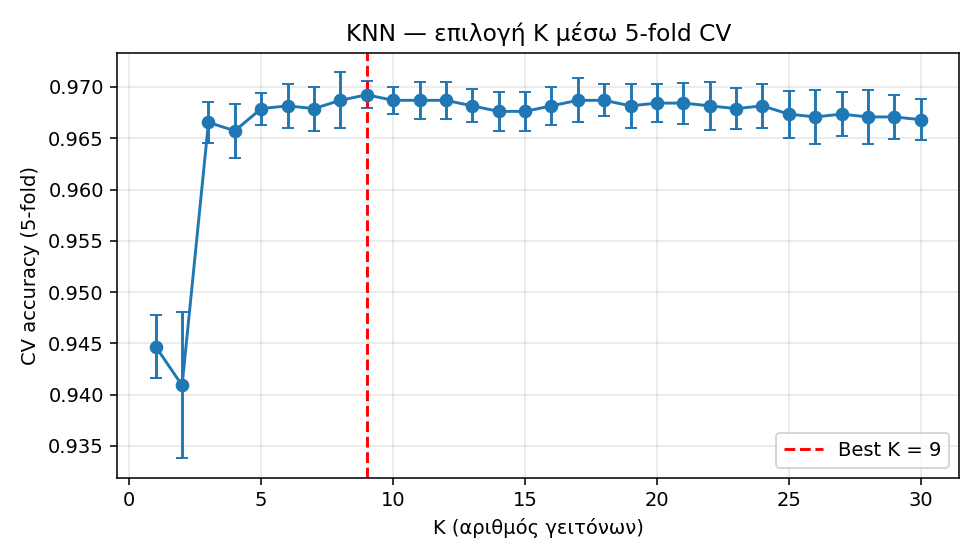
\includegraphics[width=0.9\linewidth]{Q2_knn_cv.png}
\caption{Επιλογή του \(K\) για KNN μέσω 5-fold stratified cross-validation.
Η κόκκινη διακεκομμένη γραμμή δείχνει το επιλεγμένο \(K=9\).}
\end{figure}

\section{Αποτελέσματα στο test set}

\subsection{Συνοπτικός πίνακας}

Μετά την επιλογή \(K=9\), εκπαιδεύσαμε όλες τις μεθόδους στο training
set και τις αξιολογήσαμε στο test set (30\% των δεδομένων). Ο πίνακας
που ακολουθεί συνοψίζει τα κυριότερα μέτρα ακρίβειας:

\begin{center}
{\small
\begin{tabular}{lccccc}
\toprule
Μέθοδος & Accuracy & Bal. Acc. & AUC & F1 white & F1 red \\
\midrule
KNN (\(K=9\)) & \textbf{0,9704} & \textbf{0,9614} & 0,9664 & \textbf{0,9804} & \textbf{0,9401} \\
Logistic Reg. & 0,9654 & 0,9529 & \textbf{0,9692} & 0,9771 & 0,9296 \\
LDA & 0,9679 & 0,9546 & 0,9678 & 0,9788 & 0,9344 \\
QDA & 0,9559 & 0,9415 & 0,9605 & 0,9708 & 0,9107 \\
Gaussian NB & 0,9440 & 0,9344 & 0,9575 & 0,9625 & 0,8894 \\
\bottomrule
\end{tabular}
}
\end{center}

\subsection{Σύντομη υπενθύμιση των metrics}

Επειδή οι αριθμοί είναι κοντά μεταξύ τους, αξίζει να ξαναθυμηθούμε τι
δείχνει ο καθένας πριν τους ερμηνεύσουμε:
\begin{itemize}
    \item \textbf{Accuracy}: το συνολικό ποσοστό σωστών προβλέψεων. Εδώ
    όλες οι μέθοδοι ξεπερνούν το 0,94.
    \item \textbf{Balanced accuracy}: ο μέσος όρος των recall για τις δύο
    κλάσεις (recall red και recall white). Προστατεύει από το να
    ``κρύβεται'' μια αδυναμία στην πιο σπάνια κλάση.
    \item \textbf{AUC}: πόσο καλά το μοντέλο βάζει σε σειρά τα κρασιά,
    ανεξάρτητα από το threshold. Όλες οι μέθοδοι εδώ ξεπερνούν το 0,95.
    \item \textbf{F1 white}: αρμονικός μέσος precision/recall για τα
    white.
    \item \textbf{F1 red}: αρμονικός μέσος precision/recall για τα red.
    Είναι πιο ενημερωτικό, γιατί red είναι η πιο σπάνια κλάση.
\end{itemize}

\subsection{Ερμηνεία των αποτελεσμάτων}

Από τον πίνακα προκύπτουν τρία καθαρά μηνύματα:
\begin{enumerate}
    \item \textbf{Και οι πέντε μέθοδοι λειτουργούν πολύ καλά}. Η accuracy
    είναι πάνω από 94\% σε όλες τις περιπτώσεις. Αυτό δείχνει ότι, όταν
    χρησιμοποιούμε όλες τις χημικές μεταβλητές μαζί, το πρόβλημα διάκρισης
    red από white γίνεται σχετικά εύκολο.

    \item \textbf{Ο KNN κερδίζει οριακά}. Έχει την καλύτερη accuracy
    (0,9704), την καλύτερη balanced accuracy (0,9614) και το καλύτερο
    F1 για τα red. Αυτό δεν είναι τυχαίο: ο KNN δεν υποθέτει καμία
    κατανομή ή γραμμικό όριο. Αξιοποιεί ``τοπικά'' μοτίβα στα δεδομένα
    και έτσι μπορεί να πιάσει λεπτότερες διαφορές που οι άλλες μέθοδοι
    χάνουν λόγω των υποθέσεών τους.

    \item \textbf{Το Gaussian NB πέφτει τελευταίο}. Αυτό είναι
    αναμενόμενο: το Gaussian NB υποθέτει ότι οι μεταβλητές είναι
    \emph{ανεξάρτητες μέσα σε κάθε κλάση}. Στο πρόβλημά μας αυτό δεν
    ισχύει. Για παράδειγμα, το \code{total sulfur dioxide} και το
    \code{free sulfur dioxide} είναι ισχυρά συσχετισμένα. Όταν το NB
    αγνοεί τη συσχέτιση, υπερεκτιμά την πληροφορία που δίνει το δείγμα.
\end{enumerate}

\subsection{Γιατί η QDA είναι χειρότερη από τη LDA εδώ}

Ένα σημείο που αξίζει προσοχή: η QDA είναι πιο ευέλικτη από τη LDA, αλλά
στο πρόβλημά μας είναι πιο ανακριβής (0,9559 έναντι 0,9679). Γιατί;

Ο λόγος είναι ότι στις 11 διαστάσεις η QDA πρέπει να εκτιμήσει έναν
πλήρη πίνακα συνδιακύμανσης \(\boldsymbol{\Sigma}_k\) για την κάθε
κλάση. Αυτό σημαίνει πολλές παραμέτρους (της τάξης του \(p^2/2\) για
κάθε κλάση). Όταν υπάρχουν μεταβλητές με ισχυρές συσχετίσεις (όπως οι
χημικοί δείκτες του κρασιού), αυτές οι εκτιμήσεις γίνονται ασταθείς.

Επιπλέον, στα δεδομένα μας η \emph{σχετική δομή συσχέτισης} των
μεταβλητών δεν είναι τόσο διαφορετική ανάμεσα στις δύο κλάσεις ώστε να
αξίζει ο QDA την επιπλέον πολυπλοκότητα. Η LDA, με ένα κοινό
\(\boldsymbol{\Sigma}\), πετυχαίνει ένα καλύτερο συμβιβασμό μεταξύ
``ευελιξίας'' και ``στατιστικής σταθερότητας''.

\subsection{Confusion matrices}

Για να δούμε ποιες προβλέψεις λείπουν από κάθε μοντέλο, παραθέτουμε τους
confusion matrices στο test set. Όπως και πριν:
\code{TN} = πραγματικό red ταξινομημένο ως red,
\code{FP} = πραγματικό red ταξινομημένο ως white,
\code{FN} = πραγματικό white ταξινομημένο ως red,
\code{TP} = πραγματικό white ταξινομημένο ως white.

\begin{center}
{\small
\begin{tabular}{lrrrr}
\toprule
Μέθοδος & TN & FP & FN & TP \\
\midrule
KNN (\(K=9\)) & 369 & 22 & 25 & 1173 \\
Logistic Reg. & 363 & 28 & 27 & 1171 \\
LDA & 363 & 28 & 23 & 1175 \\
QDA & 357 & 34 & 36 & 1162 \\
Gaussian NB & 358 & 33 & 56 & 1142 \\
\bottomrule
\end{tabular}
}
\end{center}

Τα συνολικά κρασιά στο test set είναι 1589, εκ των οποίων 391 είναι red
και 1198 είναι white (αναλογία \(\approx 75{:}25\), ίδια με την
συνολική).

Ο KNN κάνει σχετικά ισορροπημένα λάθη. Βρίσκει:
\begin{itemize}
    \item 369 από τα 391 red, δηλαδή recall red \(\approx 0{,}944\),
    \item 1173 από τα 1198 white, δηλαδή recall white \(\approx 0{,}979\).
\end{itemize}

Αντίθετα, το Gaussian NB κάνει σαφώς περισσότερα λάθη στα white
(56 λάθη), παρόλο που έχει αριθμό red-σωστών παρόμοιο με τις άλλες
μεθόδους. Αυτό ρίχνει την accuracy του.

\section{ROC καμπύλες και AUC}

\subsection{Η εικόνα}

Σχεδιάσαμε όλες τις ROC καμπύλες μαζί στον ίδιο άξονα για εύκολη
σύγκριση.

\begin{figure}[H]
\centering
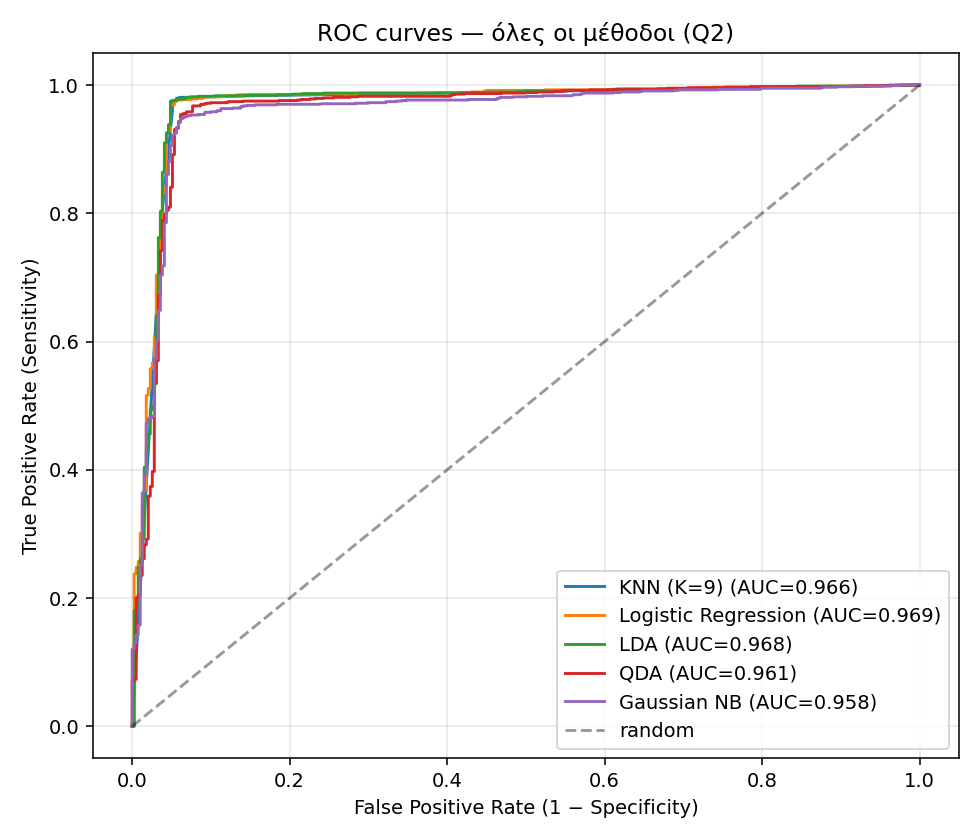
\includegraphics[width=0.95\linewidth]{Q2_roc.png}
\caption{ROC καμπύλες των πέντε μεθόδων του Ερωτήματος Β. Η διαγώνια
γραμμή αντιστοιχεί σε ένα μοντέλο που κάνει τυχαίες προβλέψεις.}
\end{figure}

Παρατηρούμε ότι και οι πέντε καμπύλες είναι αρκετά κοντά στην πάνω
αριστερή γωνία του διαγράμματος. Καμία δεν πλησιάζει τη διαγώνιο, άρα
κανένα μοντέλο δεν είναι ``τυχαίο''. Οι τιμές AUC είναι:
\begin{center}
{\small
\begin{tabular}{lc}
\toprule
Μέθοδος & AUC \\
\midrule
Logistic Regression & \textbf{0,9692} \\
LDA & 0,9678 \\
KNN (\(K=9\)) & 0,9664 \\
QDA & 0,9605 \\
Gaussian NB & 0,9575 \\
\bottomrule
\end{tabular}
}
\end{center}

\subsection{Γιατί η AUC της Logistic Regression είναι η μεγαλύτερη, αλλά
όχι η accuracy της}

Σε αυτό το σημείο υπάρχει ένα ενδιαφέρον εύρημα. Η Logistic Regression
έχει τη \emph{μεγαλύτερη} AUC (0,9692), όμως ο KNN έχει τη
\emph{μεγαλύτερη} accuracy στο test set (0,9704). Δεν είναι αντίφαση.

Θυμίζουμε ότι:
\begin{itemize}
    \item Η \textbf{AUC} μετράει πόσο καλά το μοντέλο βάζει τα δείγματα
    σε σειρά από ``πιο πιθανό white'' προς ``λιγότερο πιθανό white''.
    Άρα αντιστοιχεί στην ποιότητα των πιθανοτήτων, ανεξάρτητα από το
    threshold.
    \item Η \textbf{accuracy} αφορά την τελική ετικέτα, δηλαδή εξαρτάται
    από το συγκεκριμένο threshold (εδώ το default 0,5).
\end{itemize}

Η Logistic Regression δίνει πολύ καθαρές, καλά βαθμονομημένες
πιθανότητες, οπότε η σειρά των δειγμάτων είναι εξαιρετική (υψηλή AUC).
Ο KNN δεν έχει τόσο ``ομαλές'' πιθανότητες (αφού κάθε πιθανότητα προκύπτει
ως κλάσμα k/9), αλλά στο default threshold οι τελικές του προβλέψεις
τυχαίνει να είναι ελαφρώς καλύτερες στο συγκεκριμένο test set.

Η ουσία είναι ότι οι δύο μετρικές μετράνε διαφορετικά πράγματα και γι'
αυτό δεν χρειάζεται να συμφωνούν πάντα.

\section{Είναι στατιστικά σημαντικές οι διαφορές;}

\subsection{McNemar test}

Όπως και στο Ερώτημα Α, για να ελέγξουμε αν οι διαφορές ανάμεσα στις
μεθόδους είναι ουσιαστικές ή αν θα μπορούσαν να προκύψουν από τύχη,
χρησιμοποιούμε τον \textbf{McNemar test}. Αυτός συγκρίνει δύο μοντέλα
πάνω στα \emph{ίδια test δεδομένα} και κοιτάζει τα δείγματα όπου το ένα
μοντέλο πέτυχε και το άλλο απέτυχε.

\begin{center}
{\small
\begin{tabular}{lccc}
\toprule
Σύγκριση & A σωστό/B λάθος & A λάθος/B σωστό & p-value \\
\midrule
KNN vs LogReg & 13 & 5 & 0,0963 \\
KNN vs LDA & 9 & 5 & 0,4240 \\
KNN vs QDA & 27 & 4 & \(7{,}77 \times 10^{-5}\) \\
KNN vs Gaussian NB & 44 & 2 & \(1{,}49 \times 10^{-9}\) \\
LogReg vs LDA & 2 & 6 & 0,2891 \\
LogReg vs QDA & 21 & 6 & 0,0071 \\
LogReg vs Gaussian NB & 38 & 4 & \(3{,}54 \times 10^{-7}\) \\
LDA vs QDA & 24 & 5 & 0,0008 \\
LDA vs Gaussian NB & 42 & 4 & \(4{,}89 \times 10^{-8}\) \\
QDA vs Gaussian NB & 25 & 6 & 0,0012 \\
\bottomrule
\end{tabular}
}
\end{center}

\subsection{Τι μας λένε τα p-values}

Με κατώφλι σημαντικότητας \(\alpha = 0{,}05\):
\begin{itemize}
    \item \textbf{KNN, Logistic Regression και LDA είναι μεταξύ τους
    πρακτικά ισοδύναμοι}. Τα p-values στα ζευγάρια KNN-LogReg
    (0,0963), KNN-LDA (0,4240) και LogReg-LDA (0,2891) είναι όλα
    \(>\alpha\). Δηλαδή οι τρεις κορυφαίοι ταξινομητές δεν μπορούν να
    ξεχωριστούν στατιστικά σημαντικά σε αυτό το test set.

    \item \textbf{Η QDA είναι χειρότερη από τις τρεις κορυφαίες}. Οι
    συγκρίσεις LogReg vs QDA (p=0,0071) και LDA vs QDA (p=0,0008)
    είναι σημαντικές. Άρα η πτώση στην accuracy της QDA δεν είναι
    τυχαία.

    \item \textbf{Το Gaussian NB είναι σαφώς χειρότερο από όλες τις
    άλλες}. Όλα τα p-values που περιλαμβάνουν Gaussian NB είναι πολύ
    μικρότερα του 0,05 (το μεγαλύτερο είναι \(3{,}54 \times 10^{-7}\)).
    Άρα η υστέρηση του NB είναι στατιστικά ισχυρή.
\end{itemize}

Συνολικά η σειρά επίδοσης που προκύπτει είναι:
\[
\{\text{KNN, LogReg, LDA}\}
\;>\;
\text{QDA}
\;>\;
\text{Gaussian NB}.
\]
Μέσα στο πρώτο σύνολο οι διαφορές είναι μικρές και μη σημαντικές.

\section{Τελικά συμπεράσματα για το Ερώτημα Β}

\subsection{Υπάρχει σημαντική διαφορά στην επίδοση των μεθόδων;}

\textbf{Ναι, αλλά όχι παντού.}

Υπάρχουν τρεις κατηγορίες:
\begin{itemize}
    \item Πρώτη ομάδα: \textbf{KNN (\(K=9\)), Logistic Regression, LDA}.
    Και οι τρεις πετυχαίνουν accuracy γύρω στο 0,965--0,970 και AUC
    γύρω στο 0,967--0,969. Ο McNemar test δεν βρίσκει στατιστικά
    σημαντικές διαφορές μεταξύ τους.

    \item Δεύτερη ομάδα: \textbf{QDA}. Έχει μικρότερη accuracy
    (0,9559) και η διαφορά της από την πρώτη ομάδα είναι στατιστικά
    σημαντική.

    \item Τρίτη ομάδα: \textbf{Gaussian Naive Bayes}. Έχει τη
    χαμηλότερη accuracy (0,9440), και η διαφορά του από όλες τις άλλες
    μεθόδους είναι στατιστικά σημαντική.
\end{itemize}

\subsection{Ποια μέθοδος έχει την καλύτερη ακρίβεια;}

Με βάση την accuracy στο test set, η καλύτερη μέθοδος είναι:
\[
\boxed{\text{KNN με } K = 9}
\]
με accuracy \(0{,}9704\) και balanced accuracy \(0{,}9614\).

Ωστόσο, με βάση την AUC, η καλύτερη μέθοδος είναι η
\textbf{Logistic Regression} (AUC \(0{,}9692\)). Επειδή όμως οι διαφορές
μέσα στην κορυφαία ομάδα (KNN, LogReg, LDA) \emph{δεν είναι στατιστικά
σημαντικές}, μπορούμε να πούμε ότι και οι τρεις αυτές μέθοδοι είναι
υποψήφιες ``νικήτριες''.

Αν έπρεπε να επιλέξουμε μία μόνο μέθοδο για πρακτική χρήση, τα
κριτήρια είναι:
\begin{itemize}
    \item Αν θέλουμε το απλούστερο και πιο ερμηνεύσιμο μοντέλο,
    διαλέγουμε \textbf{Logistic Regression} ή \textbf{LDA}, γιατί
    δίνουν επίσης συντελεστές που εξηγούν τη συνεισφορά κάθε μεταβλητής.
    \item Αν θέλουμε την υψηλότερη δυνατή τελική accuracy σε αυτό το
    συγκεκριμένο test set, διαλέγουμε \textbf{KNN (\(K=9\))}.
\end{itemize}

\subsection{Γιατί το Ερώτημα Β δίνει πολύ καλύτερα αποτελέσματα από το
Ερώτημα Α}

Στο Ερώτημα Α η καλύτερη accuracy ήταν \(0{,}7923\) (Gaussian NB με
\code{chlorides}). Στο Ερώτημα Β η χειρότερη accuracy είναι \(0{,}9440\)
(Gaussian NB με όλες τις μεταβλητές).

Αυτή η τεράστια βελτίωση προέρχεται κυρίως από δύο παράγοντες:
\begin{enumerate}
    \item \textbf{Συνδυασμός πληροφορίας}. Μεταβλητές όπως το
    \code{total sulfur dioxide}, η \code{volatile acidity} και η
    \code{density} έχουν η καθεμία πληροφορία που μόνη της δεν είχαμε
    κοιτάξει. Όταν το μοντέλο τις βλέπει όλες μαζί, μπορεί να συνδυάσει
    ενδείξεις και να πάρει πολύ πιο ασφαλείς αποφάσεις.

    \item \textbf{Οριακές περιπτώσεις γίνονται ξεκάθαρες}. Στο Ερώτημα
    Α, ένα κρασί με ``ουδέτερη'' τιμή chlorides ήταν δύσκολο να
    ταξινομηθεί. Στο Ερώτημα Β, τέτοιες οριακές περιπτώσεις
    ``ξεκλειδώνονται'' γιατί κάποια άλλη μεταβλητή (π.χ.\ η πυκνότητα ή
    το sulfur dioxide) συχνά δίνει καθαρό σήμα.
\end{enumerate}

\subsection{Σύνοψη}

Η απάντηση στο Ερώτημα Β μπορεί να συνοψιστεί σε δύο γραμμές:
\begin{itemize}
    \item Και οι πέντε μέθοδοι λύνουν το πρόβλημα πολύ καλά όταν έχουν
    όλες τις χημικές μεταβλητές.
    \item Υπάρχει στατιστικά σημαντική διαφορά ανάμεσα στις τρεις
    κορυφαίες (KNN, LogReg, LDA) και τις δύο τελευταίες (QDA, Gaussian
    NB). Η \textbf{υψηλότερη τελική accuracy ανήκει στον KNN με
    \(K=9\)}, ενώ η \textbf{υψηλότερη AUC ανήκει στη Logistic
    Regression}.
\end{itemize}

\end{document}
